% interacttfssample.tex
% v1.05 - August 2017

\documentclass[]{interact}

%\usepackage{epstopdf}% To incorporate .eps illustrations using PDFLaTeX, etc.
\usepackage[caption=false]{subfig}% Support for small, `sub' figures and tables
%\usepackage[nolists,tablesfirst]{endfloat}% To `separate' figures and tables from text if required

%\usepackage[doublespacing]{setspace}% To produce a `double spaced' document if required
%\setlength\parindent{24pt}% To increase paragraph indentation when line spacing is doubled
%\setlength\bibindent{2em}% To increase hanging indent in bibliography when line spacing is doubled

\usepackage[numbers,sort&compress]{natbib}% Citation support using natbib.sty
\bibpunct[, ]{[}{]}{,}{n}{,}{,}% Citation support using natbib.sty
\renewcommand\bibfont{\fontsize{10}{12}\selectfont}% Bibliography support using natbib.sty

%\theoremstyle{plain}% Theorem-like structures provided by amsthm.sty
%\newtheorem{theorem}{Theorem}[section]
%\newtheorem{lemma}[theorem]{Lemma}
%\newtheorem{corollary}[theorem]{Corollary}
%\newtheorem{proposition}[theorem]{Proposition}

%\theoremstyle{definition}
%\newtheorem{definition}[theorem]{Definition}
%\newtheorem{example}[theorem]{Example}

%\theoremstyle{remark}
%\newtheorem{remark}{Remark}
%\newtheorem{notation}{Notation}

\begin{document}

{\Large\bf Progress this week}

{\large\bf March 22, 2020}

\begin{itemize}

\item

\end{itemize}

\vfill

\textbf{Previous word count:} 5328 \hfill \textbf{Current word count:} 

\textbf{Previous page count:} 21.5 \hfill \textbf{Current page count:} 

\pagebreak

\articletype{REVIEW ARTICLE}% Specify the article type or omit as appropriate

\title{The Integrated Nested Laplace Approximation applied to Spatial Point Process Models}

\author{
\name{Kenneth Flagg\thanks{CONTACT Kenneth Flagg. Email: kenneth.flagg@montana.edu} and Andrew Hoegh}
\affil{Montana State University, Bozeman, MT}
}

\maketitle

\begin{abstract}
This template is for authors who are preparing a manuscript for a Taylor \& Francis journal using the \LaTeX\ document preparation system and the \texttt{interact} class file, which is available via selected journals' home pages on the Taylor \& Francis website.
\end{abstract}

\begin{keywords}
INLA, spatial prediction, log-Gaussian Cox process, spatial point process
\end{keywords}


\section{Introduction}
\label{intro}
%  {\bf Introduction:} Please introduce one or more current statistical research methods that have been widely used by other discipline(s) in the Introduction section or divide the discussion into two or more subsections within this Introduction section.

% More introduction, define point process terms.

Statistical methods for spatial prediction result in a high-dimensional
inference problem that can present computational challenges, particularly for
large datasets. For instance, when the goal of statistical modeling is to
produce a graphical map of a random variable over space, the model ultimately
must be able to predict that random variable at every pixel of the image. A map
image will typically be at least several hundred by several hundred pixels, so
in total there can easily be hundreds of thousands of pixels requiring
predictions. Thus, even when a model has only half a dozen parameters, spatial
prediction may require hundreds of thousands of latent variables.

Spatial point process models further complicate the situation; in addition to
computational challenges due to a large number of latent variables and
parameters, point process models also require evaluating difficult likelihoods.
{\it (Cite some computational papers --- Baddely?)} Both maximum
likelihood and Bayesian model fitting require integrating the intensity
function over space, but the integral is generally not available in closed
form and, unlike a probability distribution, the integral over the entire
domain does not necessarily equal one.

Many methods have been introduced for modeling spatial point patterns,
including logistic regression approximations, maximum pseudolikelihood, and
Markov chain Monte
Carlo~\cite{bermanturner,baddeleyetal,baddeleyturner,moellerwaagepetersen}.
The number of parameters and latent variables in these models still poses a
major computational challenge. This computational challenge led to the
development of INLA~\cite{rueetal}.

{\it (Add a paragraph about computational challenges. This is really the point
of INLA (fast albeit approximate solutions). ---Andy)}

Development of the integrated nested Laplace approximation (INLA) has made
accurate approximate model fitting considerably more feasible for a particular
class of log-Gaussian Cox process (LGCP) models. INLA was developed to fit
Bayesian hierarchical models with many latent Gaussian
variables~\cite{rueetal}. A key part of INLA's computational simplicity is that
it calculates the posterior distribution of each latent Gaussian variable one
at a time; that is, it provides only the posterior marginal distributions
rather than the full joint distribution.

When using a LGCP for spatial mapping, two aspects make INLA a suitable
approach. First, the LGCP is driven by a spatial Gaussian process (GP), so the
latent variables are Gaussian. Second, even though the latent variables are
expected to exhibit spatial dependence, their full joint distribution is not
needed. In most situations it suffices to map their predicted values, variance,
and upper and lower interval bounds pointwise across space.

We focus on spatial mapping using a hierarchical construction of the LGCP, and
do so without discussing many classic spatial point process concepts such as
Gibbs processes, Markov processes, point process densities, or the Papangelou
conditional intensity function. For readers interested in the general spatial
point process context in which the LGCP originates, we recommend other
references~\cite{moellerwaagepetersen, digglepoint, cressie}.

{\it (paragraph about partially observed point processes --- describe both
distance sampling and subwindow observation to set up for \S\ref{veffort})}

%Much recent work in point process modeling involves spatiotemporal models,
%which are easily implemented in INLA by allowing the parameters of a spatial
%point process model to vary over time. To keep the focus on the spatial
%aspects, we do not discuss spatiotemporal models.

This article provides a review of recent advances in the fitting of spatial
LGCP models via INLA, including a finite element approach for dimension
reduction, a likelihood factorization that avoids gridding, and incorporation
of sampling effort or false negatives. The examples use a freely-available
datasets and the R code is provided in the supplementary materials.

The remainder of Section~\ref{intro} provides an overview of spatial LGCP
models and INLA. Section~\ref{methods} describes the methodology developed to
fit LGCP models in INLA, and Section~\ref{application} presents example
analyses of real-world data. Finally, Section~\ref{conclusion} presents
concluding remarks.


\subsection{Log-Gaussian Cox Process}
\label{lgcp}

%Notes from \cite{moellerwaagepetersen}
%{\it (delete once fully integrated into text)}:

%\begin{itemize}

%\item applications mentioned: seismology, ecology, forestry, geography, spatial
%epidemiology and materials science

%\item modern computing (e.g. McMC) allows for model-based inference without a
%stationarity assumption

%\item Minke whale distance sampling data used as an example of incomplete
%observation (they used a shot noise Cox process model)

%\item distribution of point process is the joint distrubition of \(n\) and
%the \(n\) events, or equivalently the distribution of the number of events in
%any arbitrary region

%\item in their presentation of the two Poisson process postulates, the second
%one is given the number of events in a region they are iid proportional to the
%intensity function

%\item Cox process is driven by a non-negative random process such that
%conditional on the driving process the Cox process is a Poisson process

%\item LGCP has no edge effects because the point process in the window is
%fully specified by the GP restricted to the window

%\item quite a bit about Gibbs processes, densities wrt stationary Poisson
%processes, and Papangelou conditional intensities \emph{(comments: The density
%was traditionally used to facilitate McMC simulation and ML fitting when the
%likelihood was not explicitly available. The conditional intensity of a
%Poisson process is the intensity function because of independence among the
%points. The hierarchical setup of the LGCP lets us work directly with a
%Poisson process so the density and conditional intensity are not needed. LGCP
%models with constructed covariate can model Gibbs processes.)}

%\item more things about infinite Gibbs and Markov processes that go over my
%head but we don't need because we deal with bounded and finite processes

%\end{itemize}

%Kenny's notation and terminology:

%\begin{itemize}

%\item process defined on \(\mathcal{D} \subset \mathbb{R}^{2}\), domain of the
%intensity function, define \(d = \mathrm{dim}(\mathcal{D})\)

%\item observation window \(\mathcal{S} \subset \mathcal{D}\)

%\item \emph{(Note: When thinking about sampling, we need to define three
%regions: the domain \(\mathcal{D}\) over which the process mathematically
%operates, the region \(\mathcal{R}\) over which inferences are desired, and
%the observed/sampled observation window \(\mathcal{S}\). The general
%relationship is \(\mathcal{S} \subset \mathcal{R} \subset \mathcal{D}
%\subset \mathbb{R}^{d}\), where all of the subset symbols taken to mean
%``subset or equal''. The ``fully surveyed'' situation is \(\mathcal{S}
%= \mathcal{R}\).)}

%\item \(\mathbf{X}\) point process on \(\mathcal{R}\),
%\(\mathbf{x} = \{x_{1}, \dots, x_{n}\}\) realized point pattern

%\item point \(x \in \mathbf{x}\) called an event

%\item intensity function \(\lambda(u)\)

%\item \(x\) event, \(s\) numerical integration node, \(u\)
%arbitrary location in \(\mathcal{D}\)

%\item \(z(u)\) a column vector of covariates/predictors at \(u\)

%\item ``point'' refers to a \(u\) unless clearly stated otherwise

%\item bold for sets and spatial processes, normal italics for spatial vectors

%\item \(y\) and variations will be used for objects derived from the point
%pattern, e.g. pseudodata

%\end{itemize}

The log-Gaussian Cox process is a Poisson process driven by a latent Gaussian
process~\cite{moelleretal}. This section provides a brief overview of the
spatial Poisson process and then presents the hierarchical construction of the
spatial LGCP.

A spatial point process generates a random set of events (points) in space.
The process is characterized primarily by its intensity function
\(\lambda(u)\), which gives the local mean number of events per unit area at
any point in space. The instensity function is nonnegative and defined on a
domain \(\mathcal{D} \subset \mathbb{R}^{2}\). The point process is observed
in a bounded window \(\mathcal{R} \subset \mathcal{D}\). The point process is
denoted \(\mathbf{X}\), and its realizations are \(\mathbf{x} = \{x_{1},
\dots, x_{n}\}\). A realized (observed) \(\mathbf{x}\) is called a point
pattern; the elements of the point pattern are the events.

The Poisson process is fully defined by its intensity function and satisfies
the following two properties \cite{moellerwaagepetersen}:
\begin{enumerate}
\item The number of events in any region \(\mathcal{B}\) follows a Poisson
distribution with mean
\(\int_{\mathcal{B}} \lambda(u)\mathrm{d}u\).
\item Given the number of events in \(\mathcal{B}\), those events are
independent and identically distributed with probability density
\(\lambda(u) / \int_{\mathcal{B}} \lambda(u)\mathrm{d}u\).
\end{enumerate}
The distribution function of a Poisson process is
\begin{displaymath}
[\mathbf{X}|\lambda]
= \frac{\exp\left[-\int_{\mathcal{R}} \lambda(u) \mathrm{d}u\right]}
{n!} \prod_{x \in \mathbf{X}} \lambda(x)
\end{displaymath}
as given in Cressie (1993) \cite{cressie}. This can be extended to include
further parameters used to define \(\lambda\), most commonly coefficients
to construct a log-linear model with covariates, or a polynomial or spline
function of the spatial coordinates.

In a Poisson process, the intensity function is a fixed parameter (or a
deterministic function of fixed parameters and covariates). In applications of
spatial point process models, this is often too simplistic because spatial
heterogeneity may be driven by other random processes with their own parameters
about which inferences are desired.

A Cox process is a generalization of the Poisson process where the intensity
function is a realization of another stochastic process. Conditional on the
intensity function, a Cox process must satisfy the two Poisson process
properties, but the intensity function can take any form. Cox processes are
commonly used to model clustering of events, such as in the classic
Neyman-Scott process where cluster centers are generated by another Poisson
process~\cite{neymanscott}. Another example is where the intensity is a
Dirichlet process mixture~\cite{taddy}. In situations where the intensity
function is less structred but exhibits spatial autocorrelation, the Cox
process can incorporate a geostatistical process. The log-Gaussian Cox process
is an example of this.

The LGCP uses a log-linear model for the intensity
\begin{displaymath}
\log\lambda(u) = \boldsymbol{\Psi}(u)
= \mathbf{z}(u)' \boldsymbol{\beta} + \mathbf{e}(u),
\end{displaymath}
where \(\mathbf{e}\) is a Gaussian process with mean 0 and covariance function
\(C(u, v)\).

Where the spatial Poisson process has a (stochastically) fixed intensity to be
estimated from data, the spatial LGCP induces a hierarchical model where the
intensity function is itself a random process to be predicted.

Badeley et. al.~(2005) and M\"{o}ller and Waagepetersen~(2007) present model
checking tools for LGCP and other spatial point process
models~\cite{baddeleyresiduals,moellerwaagepetersen}.

{\it (insert paragraph reviewing applications and uses of LGCP)}


\subsection{Integrated Nested Laplace Approximation}
\label{inla}

INLA was developed with the goal of providing fast, accurate, deterministic
approximations for posterior marginal distributions of the parameters in
latent Gaussian models~\cite{rueetal}. The setting is Bayesian generalized
additive models but is kept very general; this includes linear models, models
with nonlinear (spline, random walk, etc.) functions of predictors, and models
with temporal and/or spatial dependence. Such models commonly include many
Gaussian latent variables or parameters with Gaussian priors and relatively
few non-Gaussian parameters. The INLA approach makes repeated use of Laplace
expansion, numerical integration, and numerical search. The method has
established usefulness for LGCP~\cite{illianetal}. It is readily implemented
using the standalone INLA software or in R via the R-INLA
package~\cite{inlar}.

{\it Add a page or so walking through the algorithm.}

% Define some coherent notation, then come back and spell out the algorithm.

%- $\mathbf{y} = (y_{1}, \dots, y_{n})'$ independent Gaussian observations

%- $y_{i} \sim \mathrm{N}(\theta, \sigma^{2})$

%- $\theta \sim \mathrm{N}(\mu_{0}, \sigma_{0}^{2})$

%- $\psi = 1/\sigma^{2}$, $\psi \sim \mathrm{Gamma}(a, b)$

%- The posterior distribution of $\psi$:
%$$p(\psi|\mathbf{y}) \propto \frac{p(\mathbf{y} | \theta, \psi) p(\theta) p(\psi)}
%{p(\theta | \psi, \mathbf{y})}$$

%- Laplace approximation:
%$$\tilde{p}(\psi|\mathbf{y}) \propto \frac{p(\mathbf{y} | \theta, \psi) p(\theta) p(\psi)}
%{\tilde{p}_{G}(\theta^{*} | \psi, \mathbf{y})}$$

%Repeat for $\theta$, will depend on $\psi$

%Provides marginal posteror for one entry at a time of a vector $\boldsymbol{\theta}$


\section{Methodology}
\label{methods}
%  {\bf Methodology or Approach:} Present the method(s) and relevant applications being reviewed in this or more sections.

INLA provides an efficient computational framework for fitting Bayesian models
with latent Gaussian variables. On top of this framework, several tools are
built to further simplify the fitting of spatial LGCP models. The stochastic
partial differential equation (SPDE) approach provides dimension reduction for
the spatial GP~\cite{lindgrenetal}. The SPDE approach employs a numerical
integration scheme which can also be used to approximate the LGCP likelihood
and negate the need to grid the events into Poisson counts~\cite{simpsonetal}.
With these computational improvements, researchers are now able to efficiently
fit LGCP models to large spatial point pattern datasets and even
incompletely-observed point patterns~\cite{yuanetal}.  


\subsection{The SPDE Approach}
\label{spde}

Because the LGCP includes a Gaussian process (GP), efficient computation for
Gaussian processes is critical when working with LGCP models. The GP imposes a
dense covariance matrix on the latent variables~\cite{rinla}. For GPs with a
Mat\'{e}rn covariance function, a Gaussian Markov random field (GMRF)
approximation can simplify computation, requiring only a sparse covariance
structure.

The GMRF approximation is motivated by the fact that Gaussian fields with
Mat\'{e}rn covariances are solutions to the stochastic partial differential
equation (SPDE) below~\cite{lindgrenetal}:
\begin{displaymath}
\tau(\kappa^{2} - \Delta)^{\alpha / 2} \mathbf{e}(u) = \mathbf{W}(u),
\qquad u \in \mathbb{R}^d, \quad \kappa > 0,
\quad \alpha = \nu + d/2, \quad \nu > 0.
\end{displaymath}
Here, \(\mathbf{W}\) is a Gaussian white noise process with variance 1, and
\(\Delta\) is the Laplacian operator. The stationary solution
\(\mathbf{e}\) is a Gaussian field having a Mat\'{e}rn covariance
function with precision (inverse variance) \(\tau\),  scaling parameter
\(\kappa\) (approximately inversly proportional to the range), and smoothness
parameter \(\nu\).

Lindgren, Rue, and Lindstr\"{o}m~(2011) investigate the limit as \(\nu \to 0\) for
\(d = 2\), finding that the solution is a GMRF on a unit
lattice~\cite{lindgrenetal}. They then construct approximations for positive
integer values of \(\nu\) by \(\nu\)-fold convolution of \(\mathbf{e}\)
with itself. Finally, they use a finite element method to generalize the
approximation to arbitrary triangulations of the support. This approximation
has considerable computational benefits because the GMRF has a sparse
covariance structure; the only nodes with nonzero covariances are those
directly connected by edges in the triangulation.

The core of the SPDE approach is the finite-element GMRF representation of the
GP. This technique can approximate complicated surfaces as relatively
low-dimensional vectors via a piecewise-linear approximation.
Figure~\ref{surface} shows an example. The surface is modeled at the nodes of
the mesh. Values at points other than the nodes are found by linear
interpolation, resulting in a surface constructed from triangular faces. When
using the finite element representation to compute averages or for numerical
integration, the values at the nodes are used, and are weighted by the area
represented by the nodes~(Figure~\ref{dual}). This area is one of third the
total area of the triangles of which the node is a vertex.
{\it (Add linear algebra and basis function stuff here.)}

In practice, the SPDE approach goes as follows. Choose nodes \(s_{i}\)
at which to model \(\boldsymbol{\Psi}(s_{i})
= \mathbf{z}(s_{i})' \boldsymbol{\beta} + \mathbf{e}(s_{i})\), then build a
triangular mesh using these nodes. Typically the nodes will include locations
where data or covariates are available, then the rest will be filled in with a
Delaunay triangulation under some edge length constraints. The
\(\mathbf{e}(s_{i})\) are modeled as a GMRF where the distribution of
each \(\mathbf{e}(s_{i})\) depends only on the
\(\mathbf{e}(s_{j})\) where \(s_{i}\) and \(s_{j}\) are connected by an
edge. The GMRF representation is assumed to be a piecewise linear approximation
of the continuous Gaussian field; values of \(\mathbf{e}(s)\) for
\(s\) not in the set of nodes are predicted by linear interpolation using
the barycentric coordinates of \(s\)~(Figure~\ref{triangle}). The mathematical
form of this interpolation is very simple; for a point \(u\) inside the
triangle with vertices \(s_{1}, s_{2}, s_{3}\), the approximation is simply
\begin{displaymath}
\mathbf{e}(u) \approx \alpha \mathbf{e}(s_{1})
+ \beta \mathbf{e}(s_{2}) + \gamma \mathbf{e}(s_{3}).
\end{displaymath}

% Add comments about coarsenes/fineness of mesh.

{\it (define the dual region)}

%Computationally doable when \(Z(\mathbf{s})\) has a Mat\'{e}rn covariance with
%certain values of the smoothness parameter. Check newer references.

\begin{figure}[p]

\subfloat[Example Gaussian process realization.]
{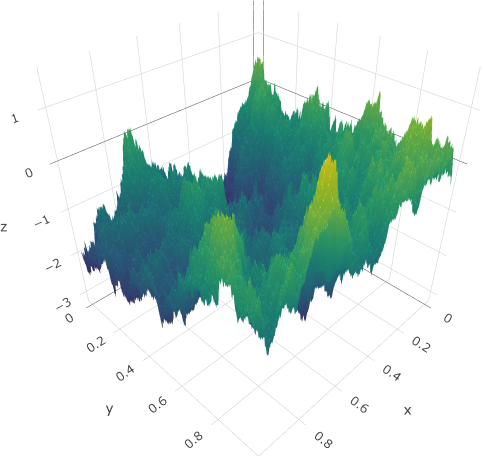
\includegraphics[width=0.5\textwidth]{figures/surface.png}}
\subfloat[Finite element approximation.]
{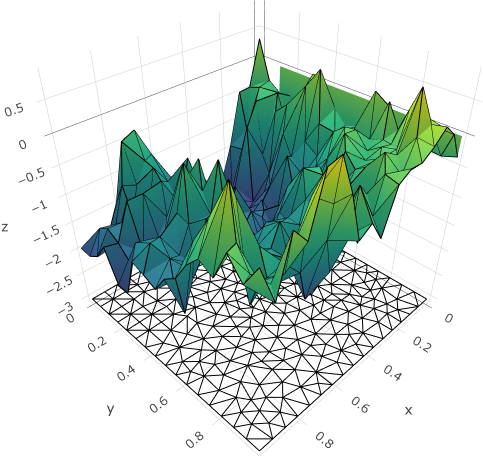
\includegraphics[width=0.5\textwidth]{figures/interp.png}}

\caption{A realization of a spatial Gaussian process and an
approximation of that realization over a triangular mesh.}
\label{surface}
\end{figure}

\begin{figure}[p]\centering
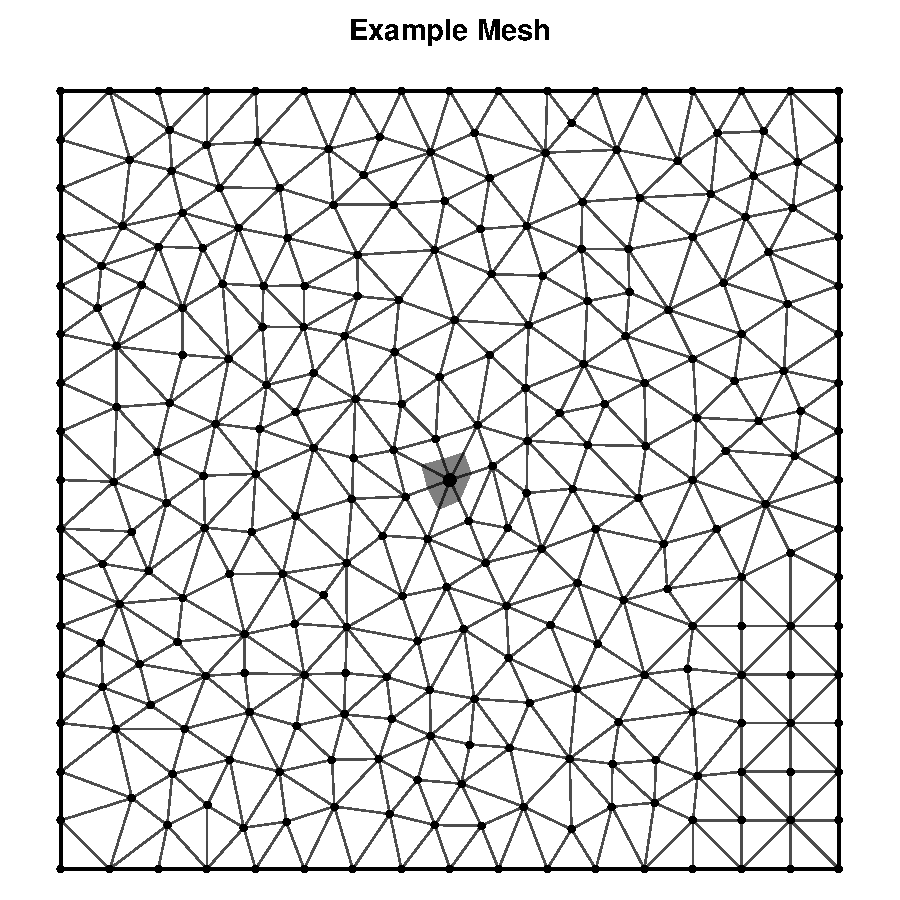
\includegraphics[width=0.5\textwidth]{figures/dual.pdf}
\caption{An illustration of the nodes (dots) and the weighting scheme for one
node (large dot). In the SPDE approach, this node represents the shaded
region, so its weight is proportional to the shaded area. The shaded region is
constructed by connecting the midpoints of the node's edges to the midpoints
of the adjacent triangles.}
\label{dual}
\end{figure}

\begin{figure}[h]\centering

\subfloat[A point \(u\) in a triangle with vertices \(s_{1}, s_{2}, s_{3}\).]
{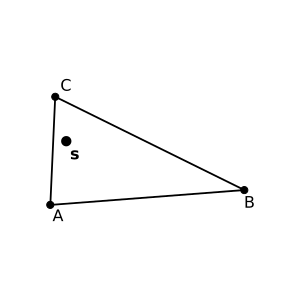
\includegraphics[width=0.4\textwidth]{figures/triangle.png}}
\hspace{2em}
\subfloat[A point \((\alpha, \beta, \gamma)\) in a simplex with vertices
\((1, 0, 0), (0, 1, 0), (0, 0, 1)\). ]
{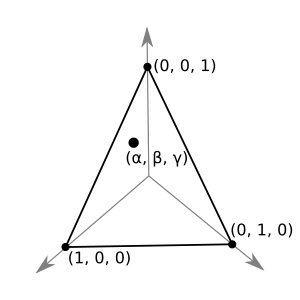
\includegraphics[width=0.4\textwidth]{figures/simplex.png}}

\caption{An illustration of the linear transformation from a mesh triangle to
the 2-simplex. The transformation is defined from \(\mathbb{R}^{2}\) to
\(\mathbb{R}^{3}\) such that the vertices are mapped to a unit vector along
each axis. This transformation takes the point \(u\) to
\((\alpha, \beta, \gamma)\), its barycentric coordinates. The barycentric
coordinates have the property that \(\alpha + \beta + \gamma = 1\).}
\label{triangle}
\end{figure}

The SPDE approach is implemented in the \texttt{INLA} package alongside tools
for constructing meshes. A wrapper for easily specifying LGCP models is
provided in the \texttt{inlabru} package~\cite{inlabru}.


\subsection{Going Off the Grid}
\label{offgrid}

Point pattern data are sometimes known as presence-only data, underscoring
the fact that information about where events did \emph{not} occur is both
important and often overlooked. There have been many proposed methods to
account for regions that were observed to contain no events (in contrast to
unobserved regions where it is unknown if any events are present). Many of
these methods involve imputation of dummy points or discretization. In the
world of maximum likelihood, perhaps the most well-developed of these use
approximations based on logistic regression on presence/absence information in
small disjoint regions {\it (cite a bunch of Baddely etc papers)}.
% What is the state-of-the-art for dummy point selection? The papers I'm
% familiar with use lattices or SRSs. Space-filling approaches?

Another alternative, which is probably the most popular approach to Bayesian
fitting of LGCP models but is also common in frequentist analyses, is to grid
the domain and model the induced Poisson counts. It has long been understood
that results are sensitive to the discretization scheme~\cite{brixmoeller}.
Simpson et. al. (2016) explain that this is also computationally
wasteful~\cite{simpsonetal}.
% Tradeoff: small grid cells for spatial precision vs small number of zeros
% for computational speed.

Simpson et. al. took LGCP inference ``off grid'' by intoducing a
computationally-efficient approximation to the Poisson process likelihood that
requires the intensity function only to be evaluated at the locations of
observed events and at the nodes of a mesh. Thus, the SPDE approach can be
employed to model the intensity surface and the same nodes reused in
evaluation of the Poisson process likelihood. The result is a substantial
improvement in both computing time and accuracy of the approximation compared
to gridding.

% Thought on efficiency: fine grid is needed for precision regarding event
% locations? Are there efficient adaptive grid methods?

The approximation arises from a factorization of the Poisson processes
likelihood. For notational clarity, assume \(\log[\lambda(u)]
= \boldsymbol{\Psi}(u)\). The exact log-likelihood is
\begin{displaymath}
\ell(\lambda) = C - \int \lambda(u) \mathrm{d}u
+ \sum_{i = 1}^{n} \log\left[\lambda(x_{i})\right]
\end{displaymath}
where \(C\) is a normalizing constant. The log-intensity is projected into the
space spanned by a finite set of basis functions,
\begin{displaymath}
\log\left[\lambda(u)\right]
\approx \sum_{j = 1}^{m} \psi_{j} \phi_{j}(u)
\end{displaymath}
with \(\boldsymbol{\psi} = (\psi_{1}, \dots, \psi_{m})'\) a multivariate
normal random vector and \(\{\phi_{1}, \dots, \phi_{m}\}\) a set of linearly
independant basis functions.
{\it (The basis function representation is actually the SPDE representation.
Say so and move this to the previous section.)}
This defines a numerical integration scheme at nodes \(s_{i}\)
with weights \(\alpha_{i}\), where the weight is the observed area represented
by the node~(Figure~\ref{dual}), and yields the approximation,
\begin{align*}
\ell(\lambda) &\approx C - \sum_{i = 1}^{m} \alpha_{i}
\exp\left[\sum_{j = 1}^{m} \psi_{j}\phi_{j}(s_{i})\right]
+ \sum_{i = 1}^{n} \sum_{j = 1}^{m} \psi_{j}\phi_{j}(x_{i}) \\
& = C - \boldsymbol{\alpha}'
\exp\left[\mathbf{A} \boldsymbol{\psi}\right]
+ \mathbf{y}' \mathbf{A}_{2} \boldsymbol{\psi}.
\end{align*}
This is equivalent to the likelihood of independent Poisson random variables
with means \(\alpha_{i} \eta_{i}\) {\it (translate the confusing algebra from
the appendix)}, and with observations \(y_{i} = 0\) at the nodes \(s_{i}\) and
\(y_{i} = 1\) at the events \(x_{i}\). Thus, the SPDE approach, which can be
easily fit in R-INLA, can be combined with a Poisson GLM to rapidly fit a LGCP
model. There is no need to compute grid counts, only to define dummy points at
the mesh nodes and construct a pseudodata vector \(\mathbf{y}\).


\subsection{Variable Sampling Effort}
\label{veffort}

There has long been a gap between point process modeling theory and practice,
where point process models are only fit to data from completely-observed
domains under the assumption that every event was detected perfectly. In
practice, this is not the case as it may be impossible or impractical to census
the entire region of interest. For example, line-transect surveys routinely
generate point pattern data but are analyzed after aggregation rather than
using a point process model. Another issue is that of false negatives, in other
words events which exist but are not detected during the survey. False
negatives are an accepted part of species abundance surveys, where the species
of interest may be camouflaged or hidden in thick cover {\it (citation?)}.

The idea of the incompletely-observed domain has been around for some time.
Brix and M\"{o}ller (2001) fit an LGCP model to weed data observed in
rectangular frames and used a Metropolis-adjusted Langevin algorthim
to predict the intensity outside of the observed frames~\cite{brixmoeller}.
Chakraborty et. al (2011) discuss nonhomogeneous Poisson process modeling as
a richer alternative to ecological presence/absence models and describe their
data as ``degraded'' in the sense that sampling bias prevented the entire
region from being fully observed; they fit their model by aggregating the
point pattern to counts in grid cells and using MCMC~\cite{chakrabortyetal}.
Gabriel et. al. (2016, 2017) derived a relationship between the Kriging
predictor and the LGCP to predict the LGCP intensity across an unobserved
subset of the region of interest~\cite{gabrieletal2016, gabrieletal2017}.

With INLA, the SPDE approach, and the ``off grid'' approximation
facilitating the routine fitting of LGCP models, there is now renewed interest
in accounting for variable sampling effort in spatial point process
models~\cite{simpsonetal,yuanetal}.

Sampling effort is accounted for using the theory of thinned point processes.
Thinning refers to the events of one point process being kept or discarded
probabilistically. Let \(\lambda(u)\) be the intensity of the parent process,
and let an event \(x=u\) (if it exists) be observed with probability
\(p(u)\). The observed point process is a thinned point process with
intensity
\begin{displaymath}
\lambda_{p}(u) = p(u) \lambda(u),
\end{displaymath}
and if the parent process is a Poisson process then the observed process is
also a Poisson process~\cite{moellerbook}.

We seek to make posterior inferences about the parent intensity,
\(\lambda(u)\). If \(p(u)\) is known, its value at each node is used to
adjust the SPDE integration weights. Most usefully, if it is known that
\(p(s) = 0\) at certain nodes \(s\) because they were outside the surveyed
domain, the weights become zero so those nodes do not contribute to the
integral. More generally, when a known subdomain is surveyed, \(p(u)\) is
an indicator function for \(u\) being in the surveyed region. When \(p(u)\)
is known, the integration weight for node \(s_{i}\) is multiplied by
\begin{displaymath}
\int_{\mathrm{dual}(s_{i})} p(u) \mathrm{d}u
\end{displaymath}
which, for indicator functions, is simply the proportion of the dual region
that is inside the surveyed region.

If \(p(u)\) is unknown, it can be modeled. Taking the logarithm of
the thinned intensity and substituting in the basis function representation,
we have the log-linear model
\begin{displaymath}
\log\left[\lambda_{p}(u)\right]
= \log\left[p(u)\right] + \sum_{j = 1}^{m} \psi_{j} \phi_{j}(u).
\end{displaymath}
Thus, any log-linear model for \(p(u)\) that can be fit by INLA and the SPDE
approach can be incorporated into the LGCP model. This provides a convenient
way to estimate the detection function from distance sampling data; the model
for \(\log(p(u))\) includes the distance to the nearest transect as a
covariate. For example, Yuan et. al (2017) fit such a model to data from a
line-transect survey using a spline model to account for the unknown detection
function~\cite{yuanetal}.


\section{Applications}
\label{application}
%  {\bf Application of your Methodology:} Present some applications of the reviewed methods to some recent data in this or more sections. Also note: Simulation studies can be presented as a sub-section in this section or in a new standalone section.


\subsection{Beilschmiedia Pendula Lauraceae Dataset}
\label{beianalysis}

For an example analysis of real-world data, we consider the locations of
\(n = 3605\) \emph{Beilschmiedia pendula Lauraceae} trees in a 1000~meter by
500~meter plot in a tropical rainforest on Barro Colorado Island,
Panama~\cite{moellerwaagepetersen}. The data are available as the \texttt{bei}
dataset in the \texttt{spatstat} R package~\cite{spatstat}. The point pattern
is accompanied by elevation and gradient covariates measured on a square
lattice with 5 m spacing. The point pattern exhibits inhomogeneity which
appears to be associated with elevation and the elevation
gradient~(Figure~\ref{bei}).


\subsubsection{Model Specification}

We use the log-Gaussian Cox process model with intensity
\begin{displaymath}
\log\left[\lambda(u)\right] = \beta_{0} + \beta_{1} z_{1}(u)
+ \beta_{2} z_{2}(u) + \mathbf{e}(u)
\end{displaymath}
where \(z_{1}(u)\) is the elevation at \(u\), \(z_{2}(u)\) is the magnitude of
the elevation gradient at \(u\), and \(\mathbf{e}(u)\) is a zero-mean Gaussian
process with Mat\'{e}rn covariance and \(\alpha = 2\).

The prior distributions are set as follows. \(\beta_{0}\), \(\beta_{1}\), and
\(\beta_{2}\) are independent \(\mathrm{N}(0, \infty)\). For the Mat\'{e}rn
covariance parameters, R-INLA provides a PC prior defined in terms of the
standard deviation \(\sigma\) and the effective range \(\rho\). The PC prior
implements is specified by defining a tail probability for each parameter. We
set \(\mathrm{Pr}(\sigma > 1) = 0.5\) to be relatively uninformative for the
SD of a log-scale random effect, and \(\mathrm{Pr}(\rho < 45) = 0.5\) similar
to the prior used by M\"{o}ller and Waagepetersen~\cite{moellerwaagepetersen}.

\begin{figure}[p]

\subfloat[Locations of trees (events).]
{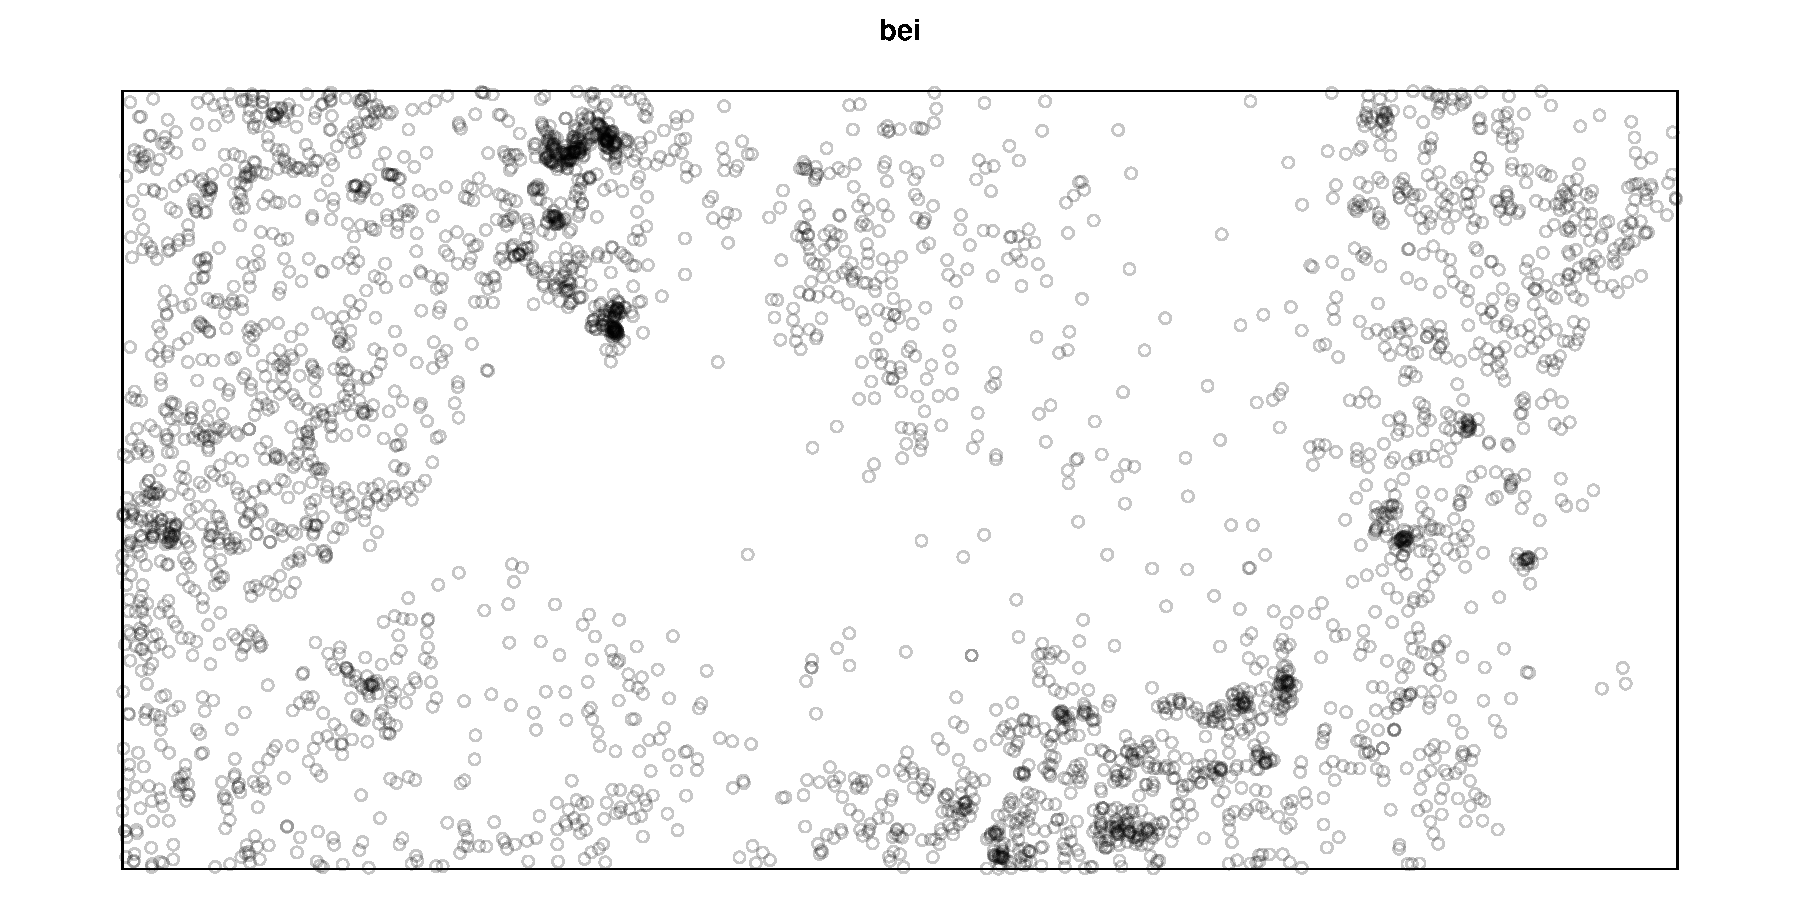
\includegraphics[width=0.9\textwidth]{figures/bei.pdf}}

\subfloat[Elevation in meters, with events overlaid.]
{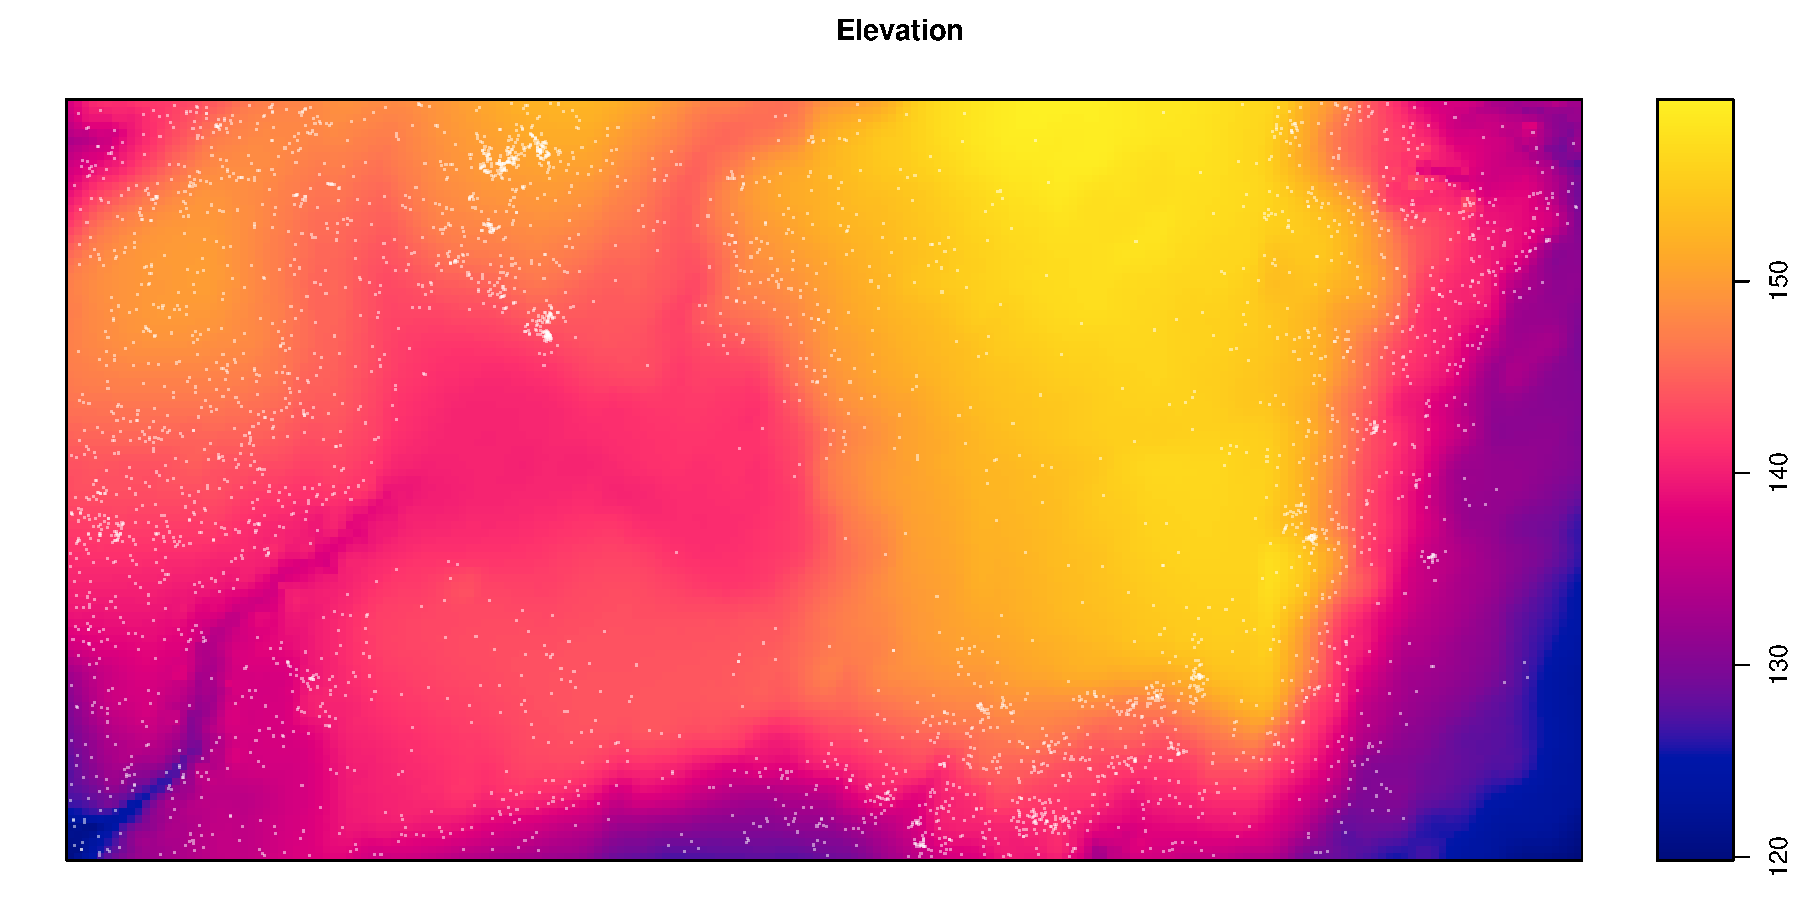
\includegraphics[width=0.9\textwidth]{figures/bei_elev.pdf}}

\subfloat[Magnitude of the elevation gradient, with events overlaid.]
{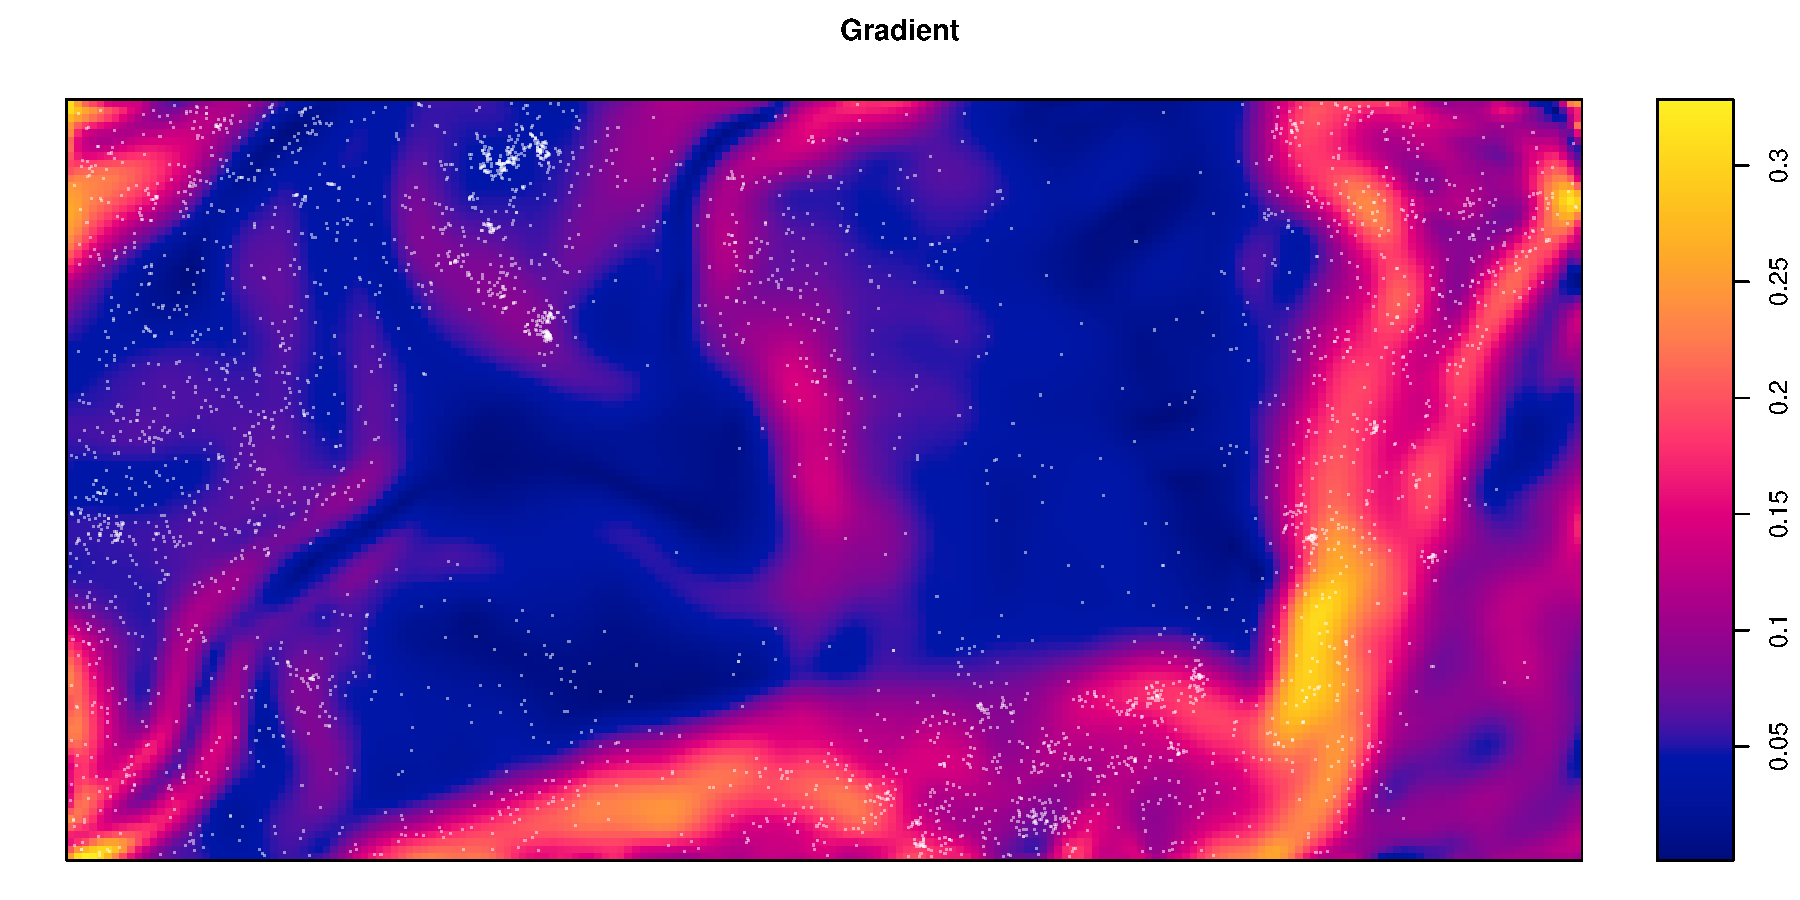
\includegraphics[width=0.9\textwidth]{figures/bei_grad.pdf}}

\caption{Plots of the event and covariate data.}
\label{bei}
\end{figure}


\subsubsection{Fitting in R-INLA}

We fit the model in R using the \texttt{INLA} package and its implementation of
the SPDE approach. Some manual preprocessing was needed to employ the Poisson
factorization. Our R code can be found in the supplementary materials. This
section provides a conceptual explanation of the model-fitting process.

The first task is to construct a mesh for the piecewise linear approximations.
A 25 meter resolution appears adequate to accurately represent the covariate
surfaces. We used tools in the \texttt{INLA} package to create a Delaunay
triangulation with a maximum edge length of 25~m. The resulting mesh has
\(m = 2145\) nodes \(s_{1},  \dots, s_{2145}\) and 4096
triangles~(Figure~\ref{beimesh}). We used linear interpolation to approximate
the covariates \(z_{1}(s_{i})\) and \(z_{2}(s_{i})\) at each node. After
creating the mesh, we specifiy the priors for the covariance parameters and
\texttt{INLA} can initialize an object to represent the covariance structure
on the mesh.

\begin{figure}[h]
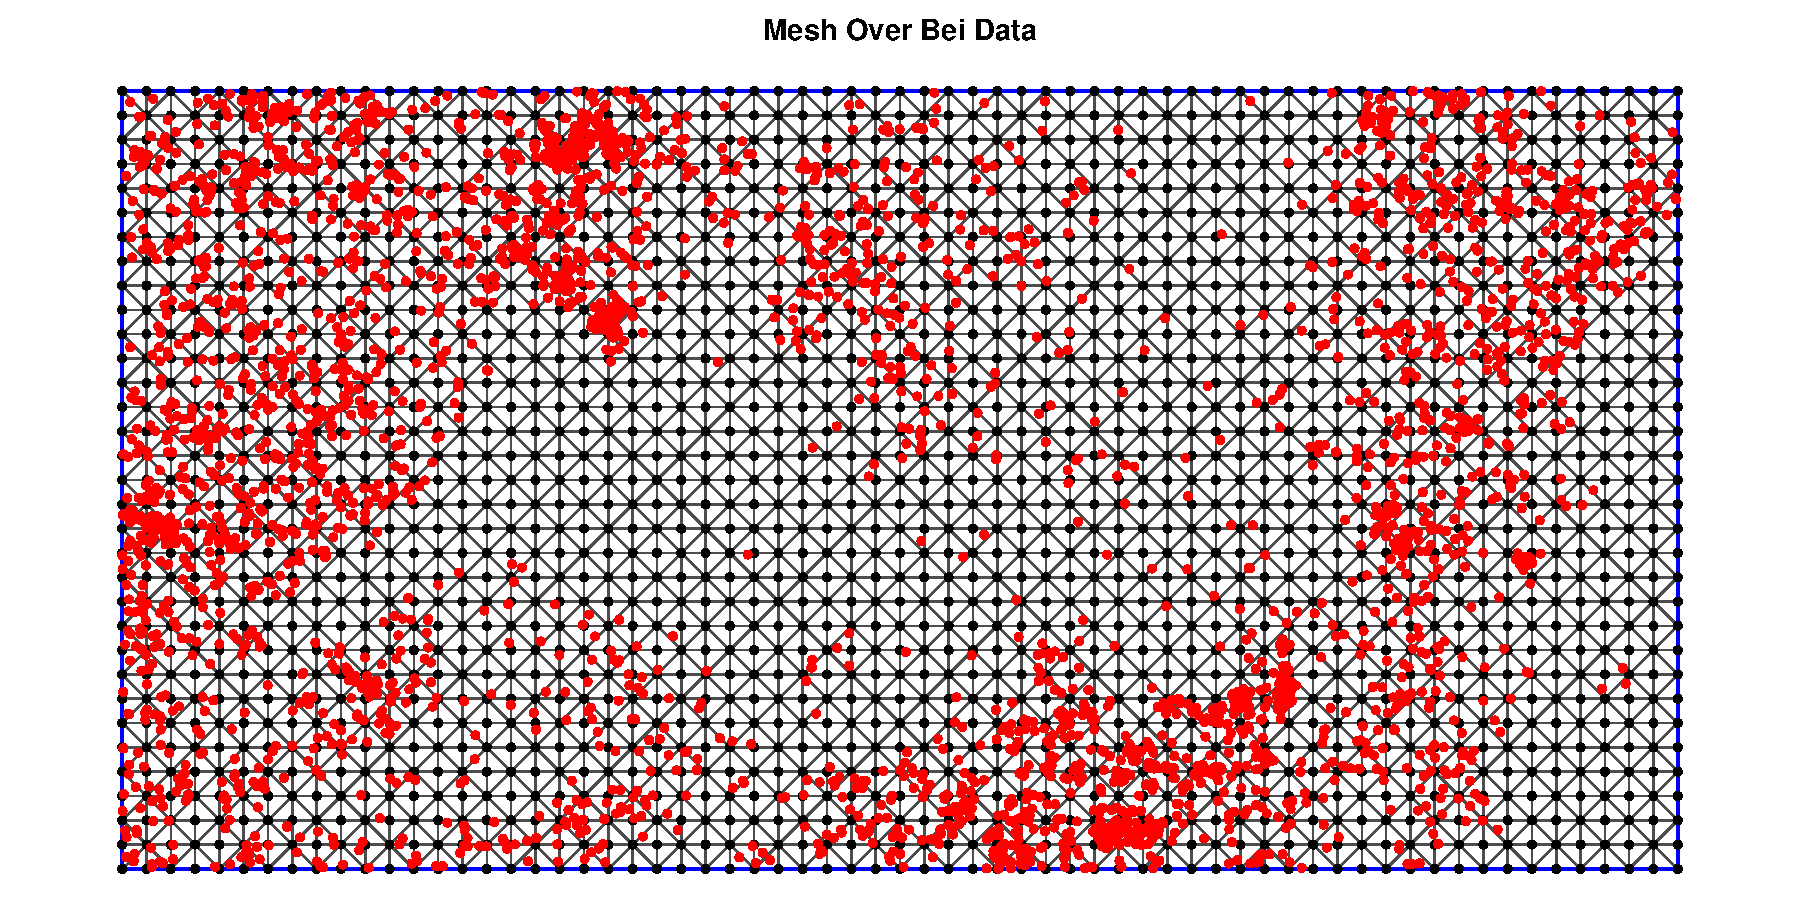
\includegraphics[width=\textwidth]{figures/bei_mesh.pdf}
\caption{Triangular mesh with pseudodata overlaid. Black dots represent
pseudodata with values of 0 at the mesh nodes. Red dots represent pseudodata
with values of 1 at the events.}
\label{beimesh}
\end{figure}

\begin{figure}[h]
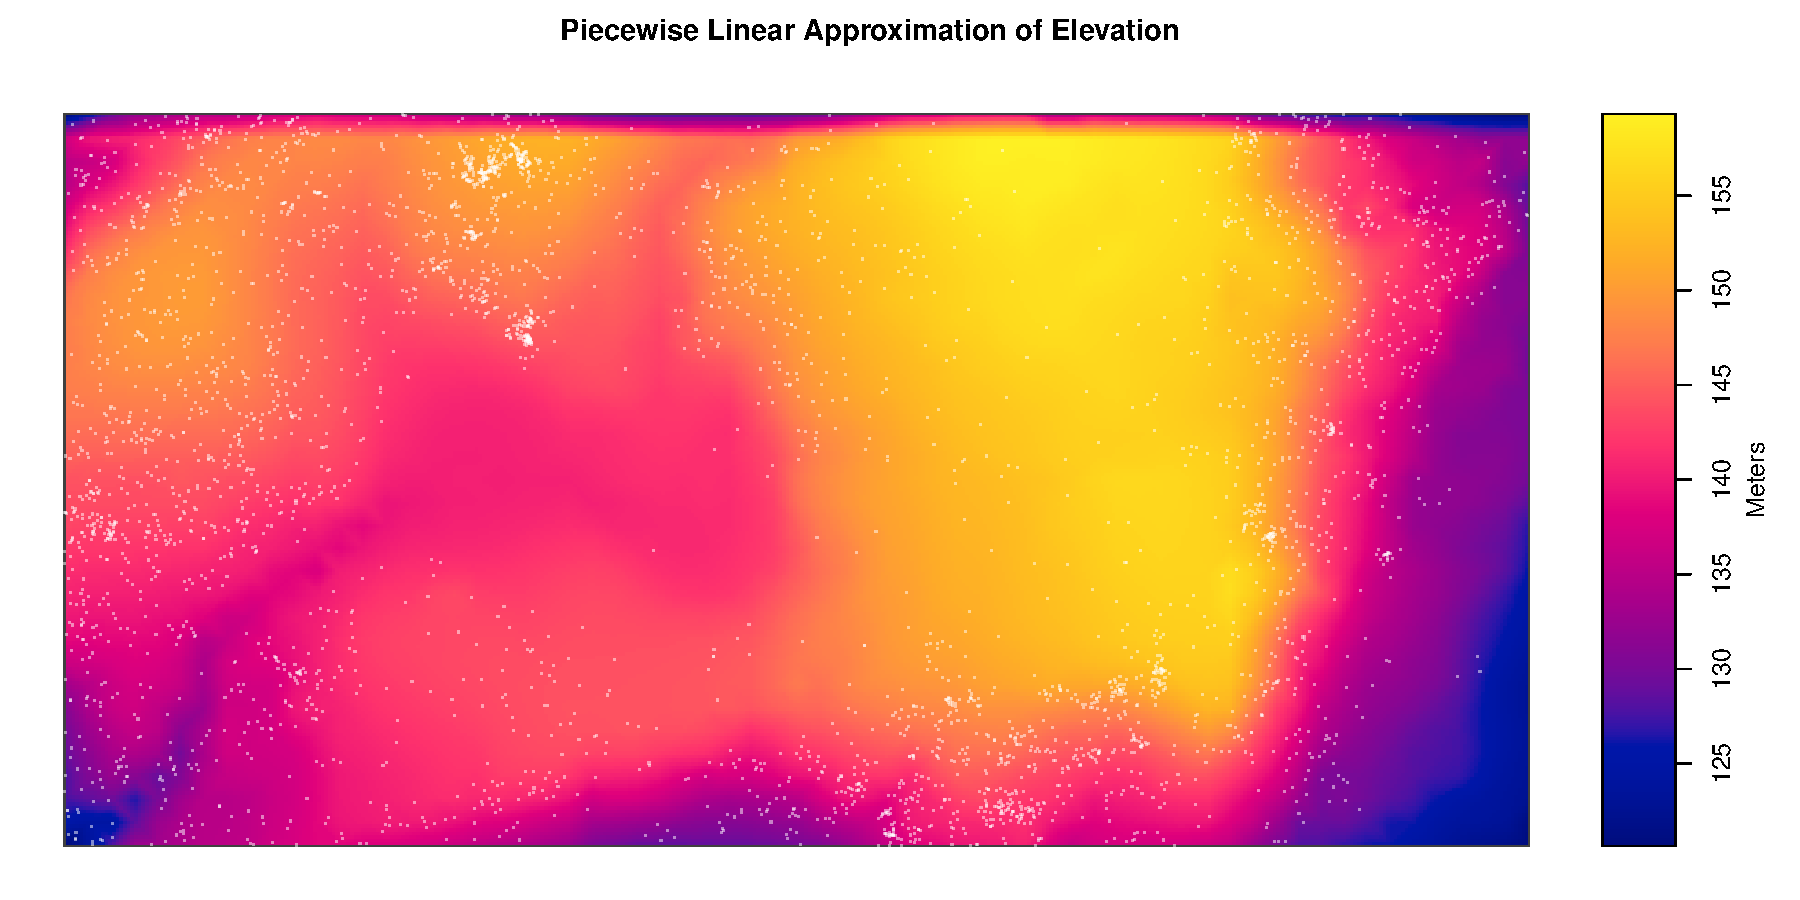
\includegraphics[width=\textwidth]{figures/bei_elev_mesh.pdf}
\caption{Piecewise linear approximation of the elevation surface.}
\label{beielevmesh}
\end{figure}

\begin{figure}[h]
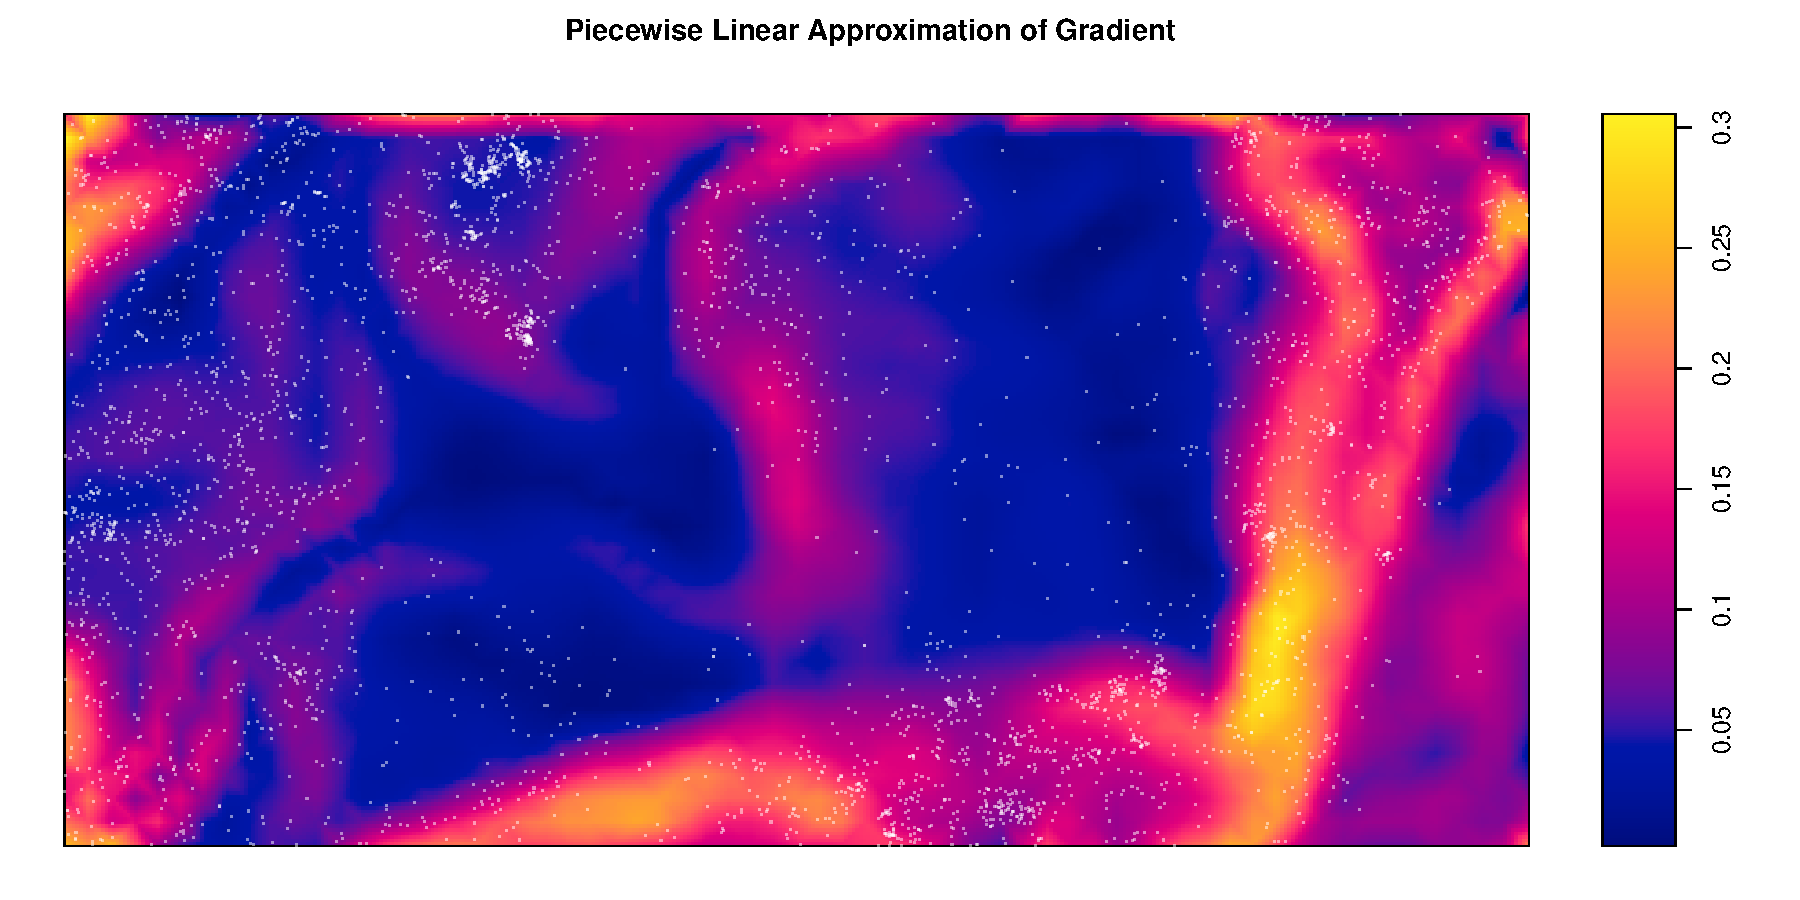
\includegraphics[width=\textwidth]{figures/bei_grad_mesh.pdf}
\caption{Piecewise linear approximation of the gradient surface.}
\label{beigradmesh}
\end{figure}

The next step is to define the pseudodata and calculate the numerical
integration weights. The pseudodata vector is
\begin{displaymath}
\mathbf{y} = (0, \dots, 0, 1, \dots, 1)'
\end{displaymath}
consisting of 2145 zeros corresponding to the mesh nodes and 3604 ones
representing the events. The weight vector is
\begin{displaymath}
\boldsymbol{\alpha} = (\alpha_{1}, \dots, \alpha_{2145}, 0, \dots, 0)'.
\end{displaymath}
The alphas equal one-third of the total area of all triangles of which each
node is a vertex, calculated by the \texttt{INLA} package. The zeros
correspond to the 3604 events, which do not contribute to the numerical
integration.

{\it Talk about the \(\mathbf{A}\) matrix.}

The final bit of setup is to combine the pseudodata, covariates at the nodes,
and a node index variable into a data list for the \texttt{inla()} function.
This function is then called with arguments specifying a formula for the
linear predictor, a Poisson family model (which defaults to a log link), the
data list, the \(\mathbf{A}\) matrix, the priors for the coefficients, and the
\(\boldsymbol{\alpha}\) vector as the exposure parameter.


\subsubsection{Results}

Posterior means and central 95\% posterior intervals:
\(\beta_{0}\): \(10.9\), \((-14.2, -7.61)\);
\(\beta_{1}\): \(0.0327\), \((0.0111, 0.0547)\);
\(\beta_{2}\): \(4.43\), \((2.41, 6.45)\);
\(\sigma\): \(1.31\), \((1.06, 1.65)\);
Range: \(178\), \((138, 234)\)

{\it decide which of figures \ref{beibetas}, \ref{beimean}, \ref{beisd},
\ref{beiintensity} are needed, then combine into a single multi-panel figure.}

The posterior mean of the fixed effect component of the linear predictor,
\begin{displaymath}
E(\beta_{0} | \mathbf{x}) + E(\beta_{1} | \mathbf{x}) z_{1}(u)
+ E(\beta_{2} | \mathbf{x}) z_{2}(u),
\end{displaymath}
appears as an average of the elevation and gradient
surfaces~(Figure~\ref{beibetas}). The fixed effects do not explain all of the
heterogeneity of the point pattern; some spatial structure remains to be
described by the posterior predicted GP~(Figure~\ref{beimean}).

\begin{figure}[h]
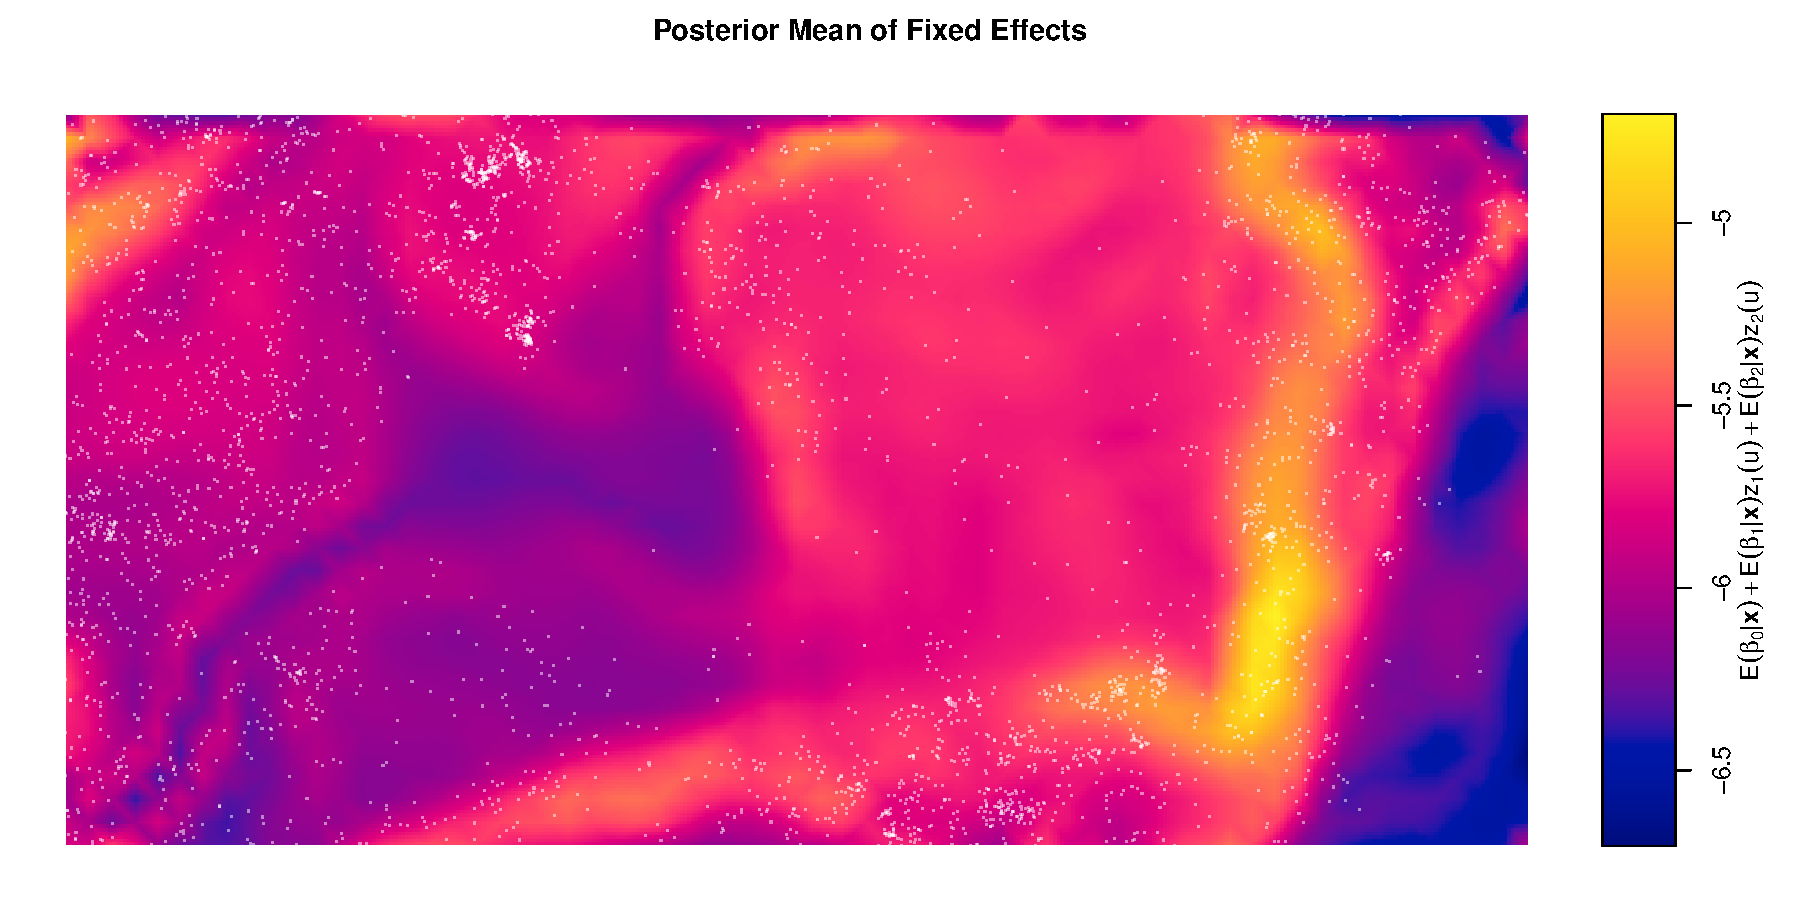
\includegraphics[width=\textwidth]{figures/bei_betas.pdf}
\caption{Posterior mean surface for the fixed effects.}
\label{beibetas}
\end{figure}

\begin{figure}[h]
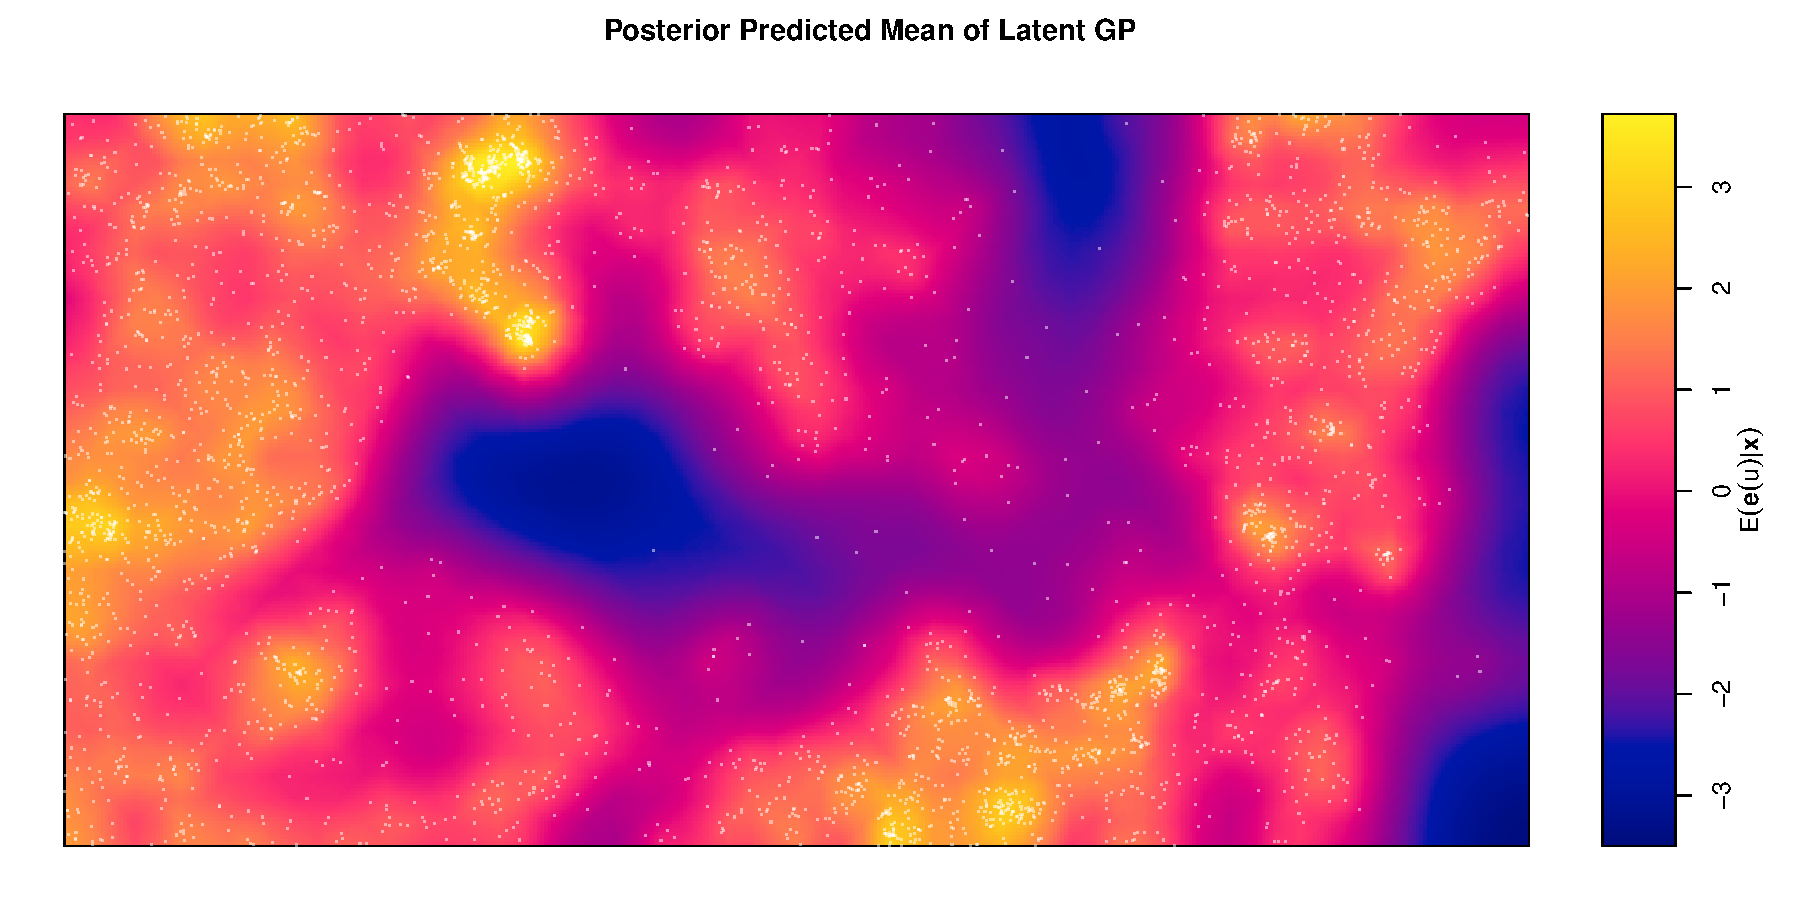
\includegraphics[width=\textwidth]{figures/bei_mean.pdf}
\caption{Posterior mean of prediction surface.}
\label{beimean}
\end{figure}

\begin{figure}[h]
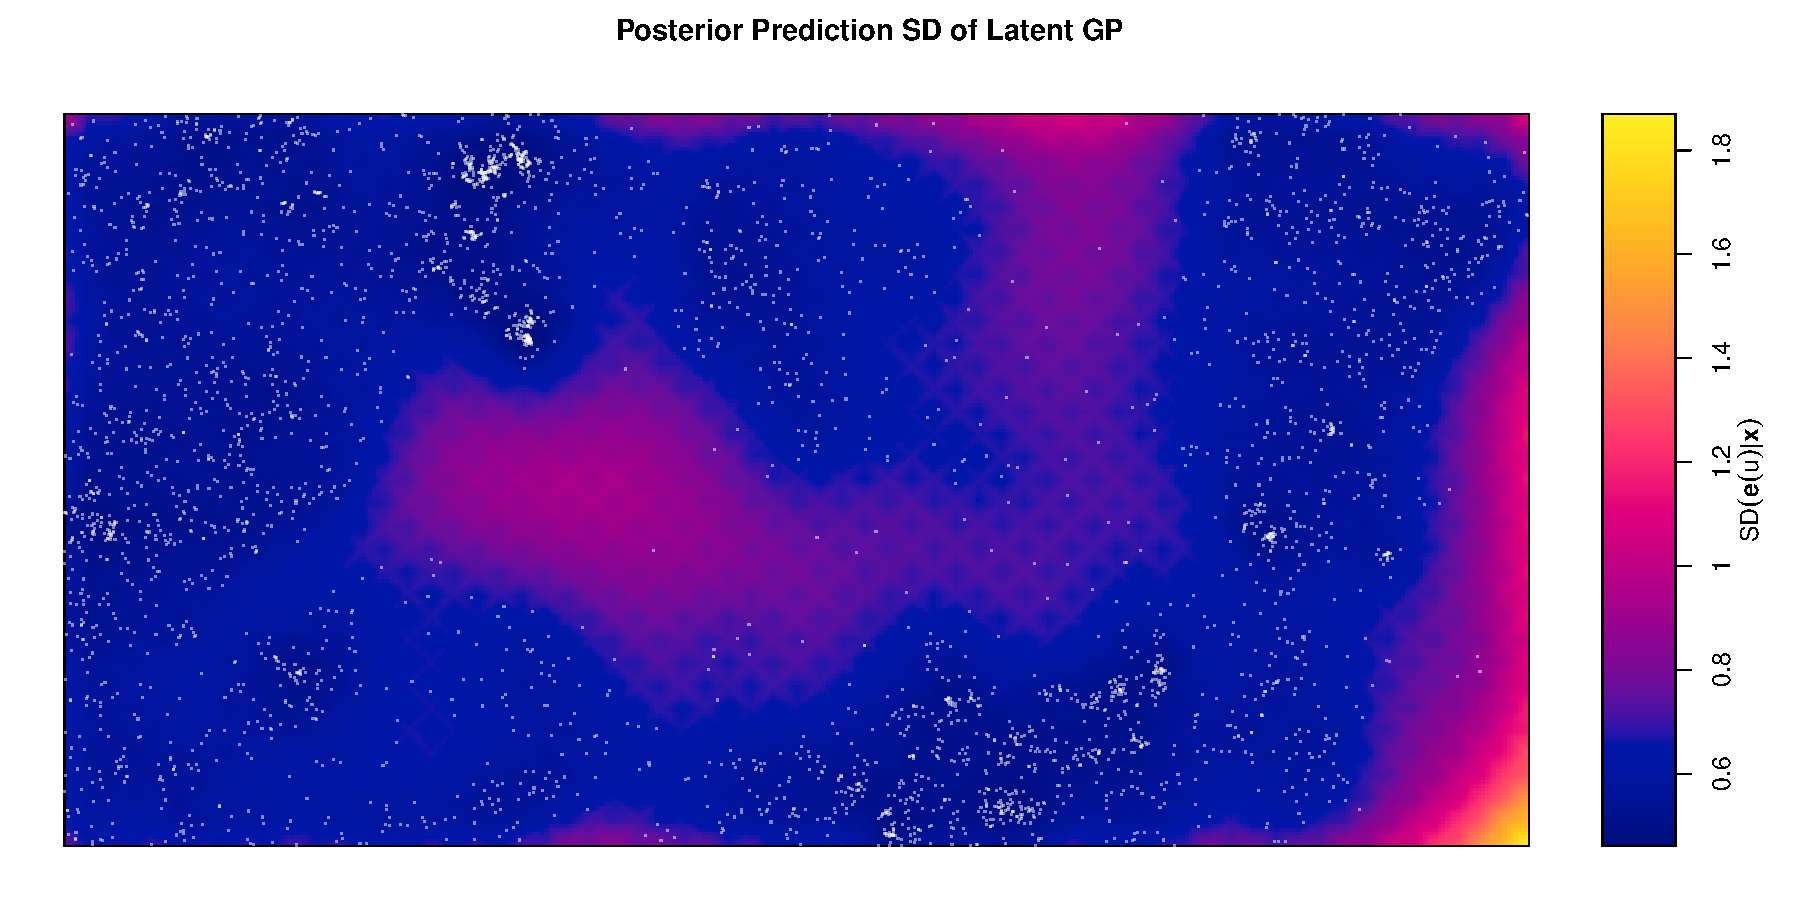
\includegraphics[width=\textwidth]{figures/bei_sd.pdf}
\caption{Pointwise posterior standard deviation of predictions.}
\label{beisd}
\end{figure}

\begin{figure}[h]
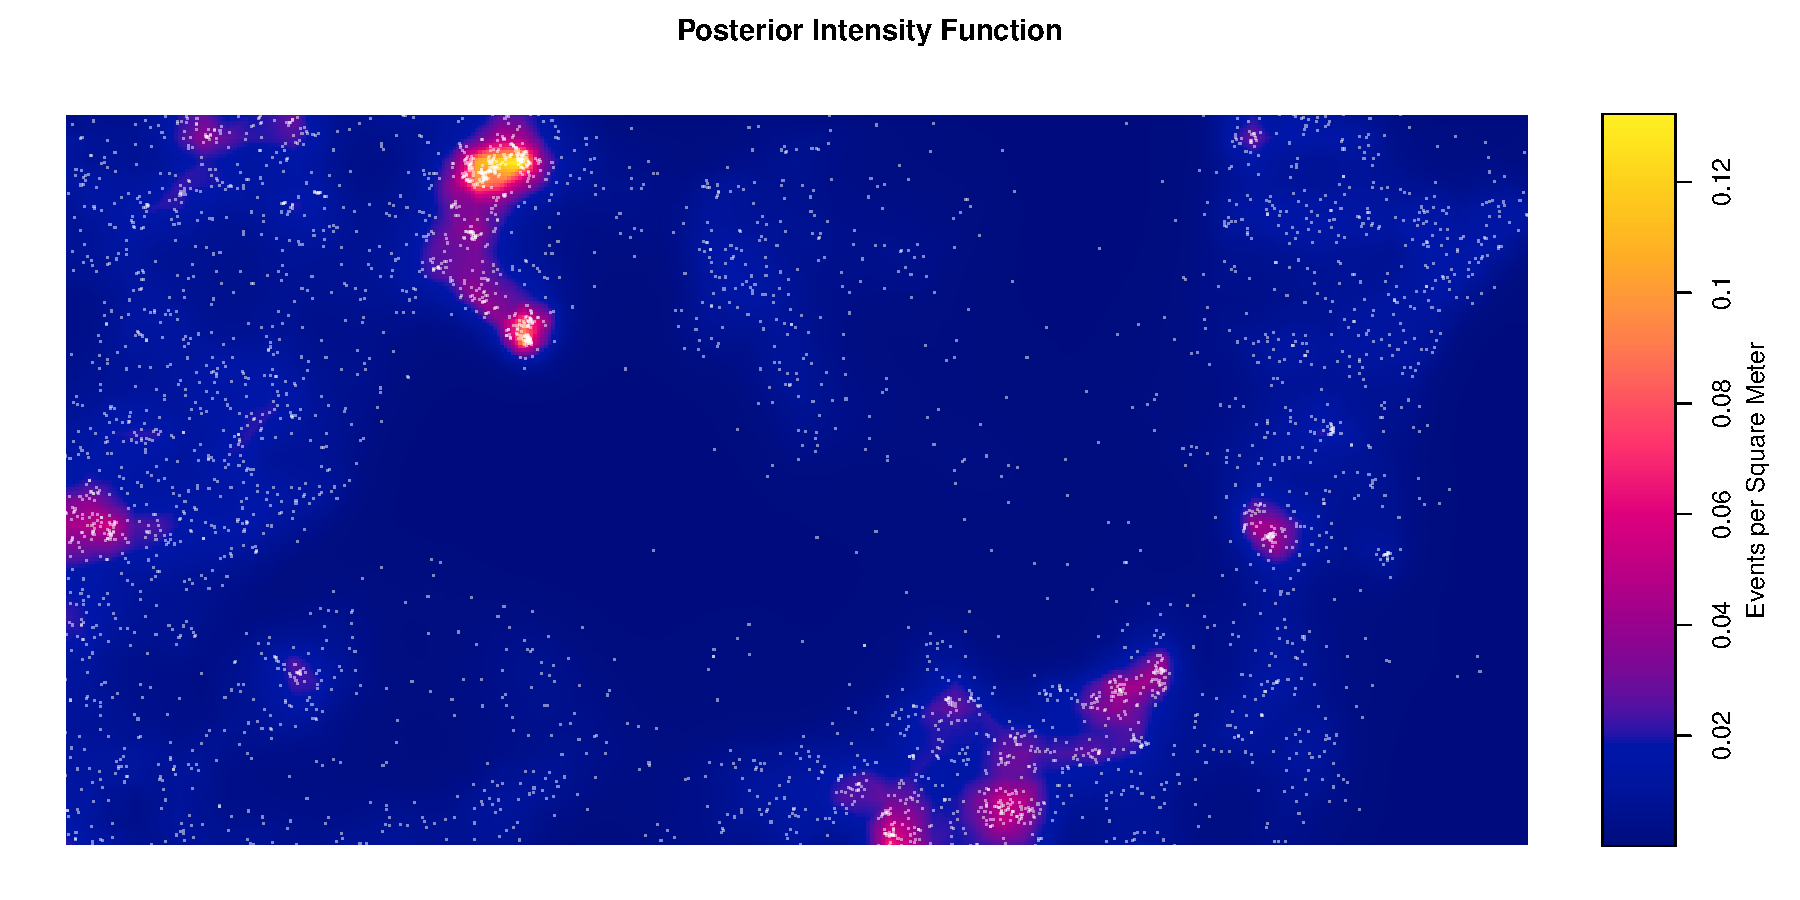
\includegraphics[width=\textwidth]{figures/bei_intensity.pdf}
\caption{Posterior intensity surface in events per square meter, calculated
using the piecewise linear approximate covariate surfaces and the posterior
means of the intercept, coefficients, and GP.}
\label{beiintensity}
\end{figure}


\subsubsection{Model Checking}

\begin{figure}[h]
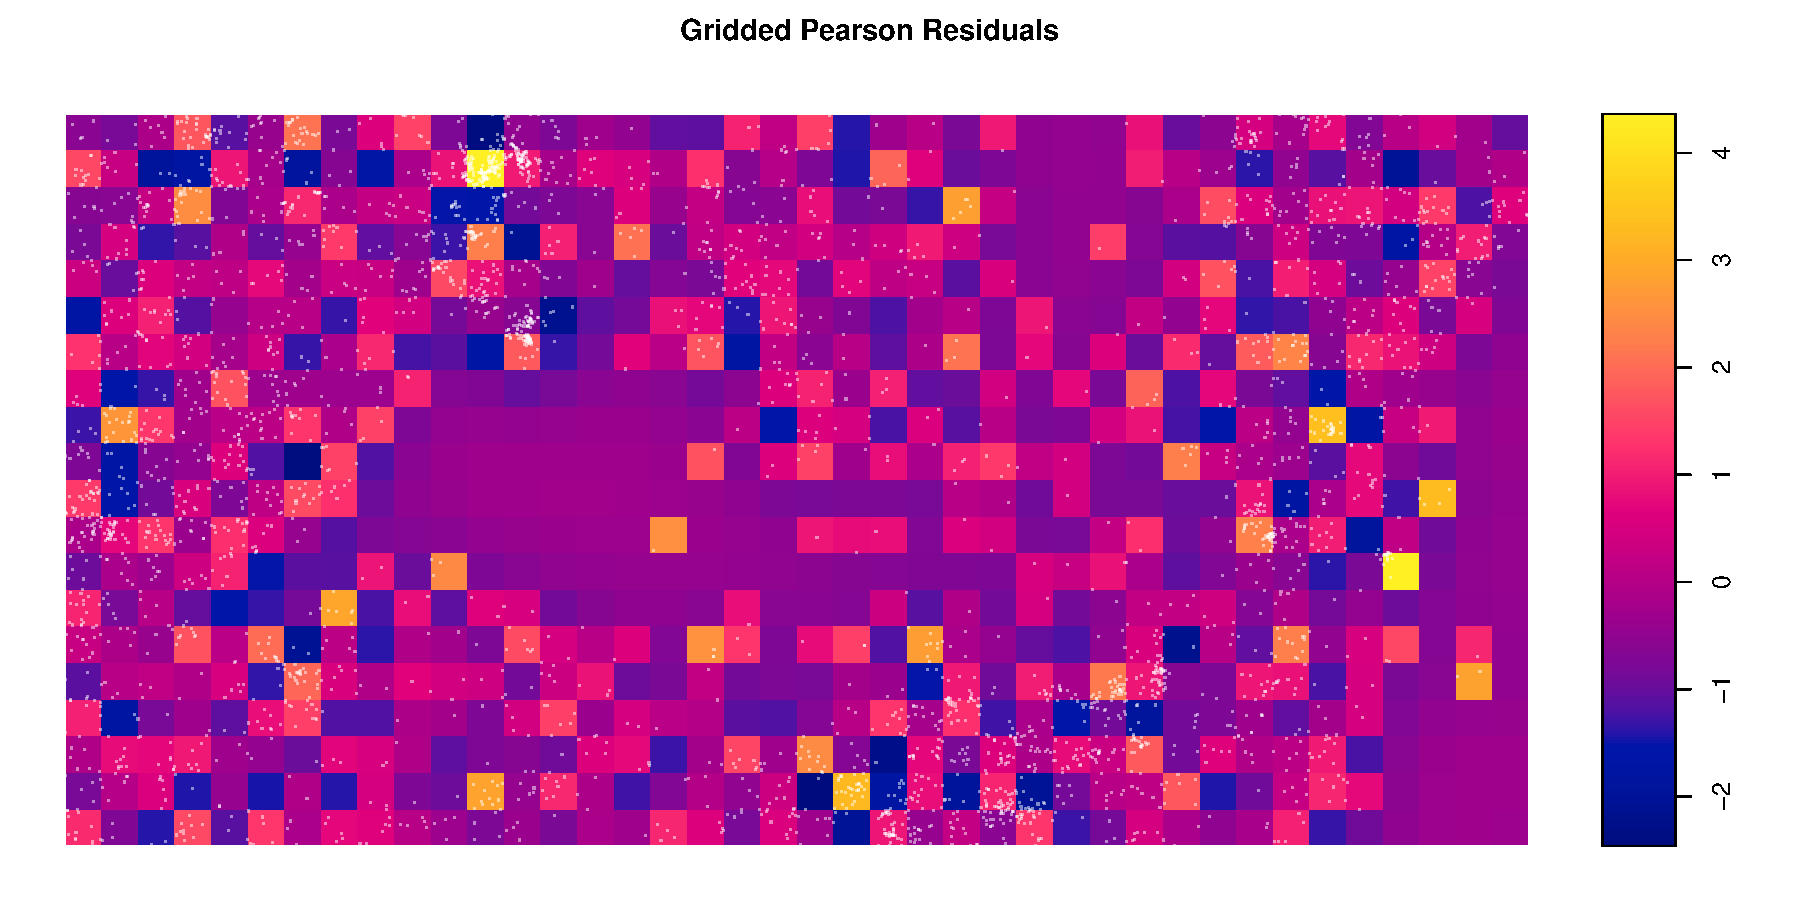
\includegraphics[width=\textwidth]{figures/bei_residuals.pdf}
\caption{Pearson residuals calculated on a grid.}
\label{beiresiduals}
\end{figure}

For a more general discussion of residuals, see \cite{baddeleyresiduals}. The
classic Pearson residual,
\begin{displaymath}
\frac{\text{Observed count} - \text{Expected count}}
{\sqrt{\text{Expected count}}},
\end{displaymath}
is a special case.

{\it Should make the whole four-panel plot if citing Baddeley et. al.}

Pearson residuals~(Figure~\ref{beiresiduals}): small magnitude in the region
with no observed events and low posterior intensity (not possible to see much
variation), the model overestimates the intensity in the canyon (too small to
be accurately represented on the mesh), random with no obvious spatial patterns
elsewhere, a few large-magnitude positive residuals (maybe there is some
clustering?), tried a few different grids (not shown) and saw the same patterns


\subsection{Transect Sampling Example}
\label{xsectanalysis}

In this section, we illustrate the analysis of incompletely-observed point
pattern data using the \emph{Beilschmiedia pendula Lauraceae} and a simulated
transect sampling scheme. Suppose part of the study requires every observed
tree to be visited so time-consuming measurements can be made on each. For
practical reasons, the researchers decide to take a systematic sample of
transects and limit data collection to events within 5~m of a transect.
Sections of the site farther than 5~m from a transect are unobserved, meaning
events in those regions cannot be observed and nothing is known about the
number of events or their locations. We assume the elevation and gradient data
were available from another source so that the full covariate data can be used
to predict the intensity in the unobserved parts of the site.

We simulate this by choosing a random starting point and defining transects
running north-south spaced 50~m apart. All events within 5~m of a transect are
saved; all other events are discarded. The result is \(n = 710\) events
observed in 20 rectangles sized 500~m by 10~m~(Figure~\ref{effort}).

{\it (the coding is more involved for the window approach than for distance
sampling --- mention a distance sampling example is in the online supplement
but the preprocessing and model-fitting procedure is not much more complicated
than for the fully-observed situation)}


\subsubsection{Model Specification}

We use the same model as fit to the full data, a log-Gaussian Cox process model
with intensity
\begin{displaymath}
\log\left[\lambda(u)\right] = \beta_{0} + \beta_{1} z_{1}(u)
+ \beta_{2} z_{2}(u) + \mathbf{e}(u).
\end{displaymath}
As before, \(z_{1}(u)\) is the elevation at \(u\), \(z_{2}(u)\) is the
magnitude of the elevation gradient at \(u\), and \(\mathbf{e}(u)\) is a
zero-mean Gaussian process with Mat\'{e}rn covariance and \(\alpha = 2\).
The prior distributions are again \(\beta_{0}\), \(\beta_{1}\), and
\(\beta_{2}\) independent \(\mathrm{N}(0, \infty)\),
\(\mathrm{Pr}(\sigma > 1) = 0.5\), and \(\mathrm{Pr}(\rho < 45) = 0.5\).

\begin{figure}[p]

\subfloat[Locations of observed trees (events).]
{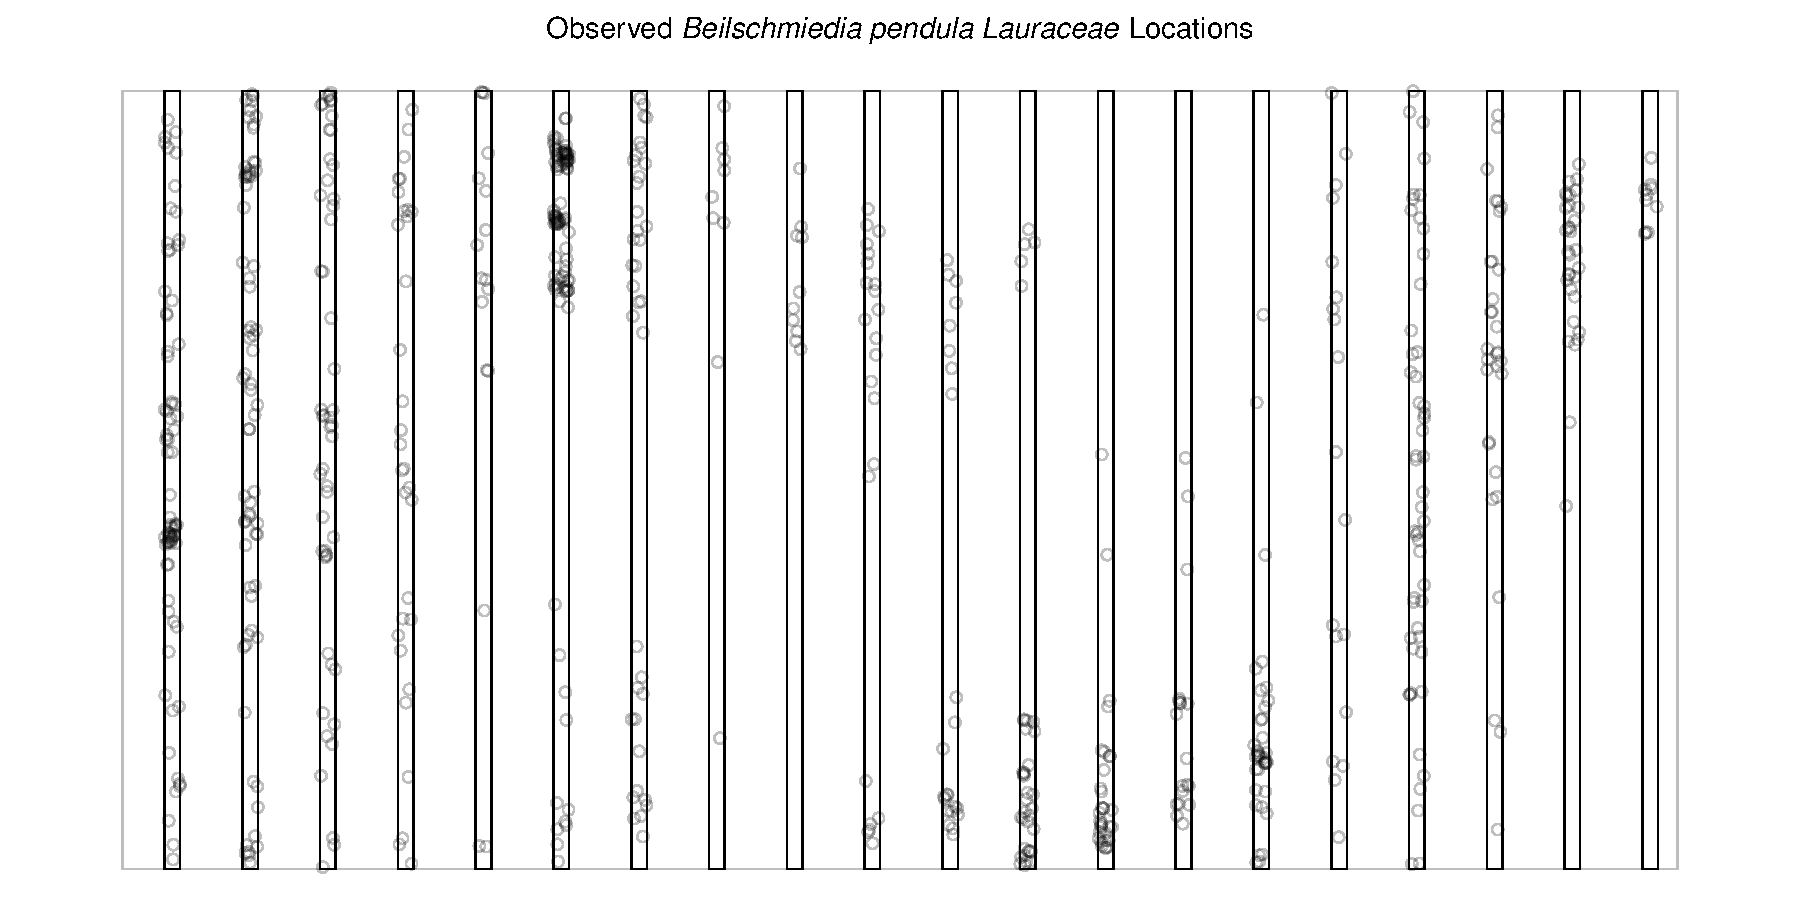
\includegraphics[width=0.9\textwidth]{figures/bei-effort.pdf}}

\subfloat[Elevation in meters, with observed region and events overlaid.]
{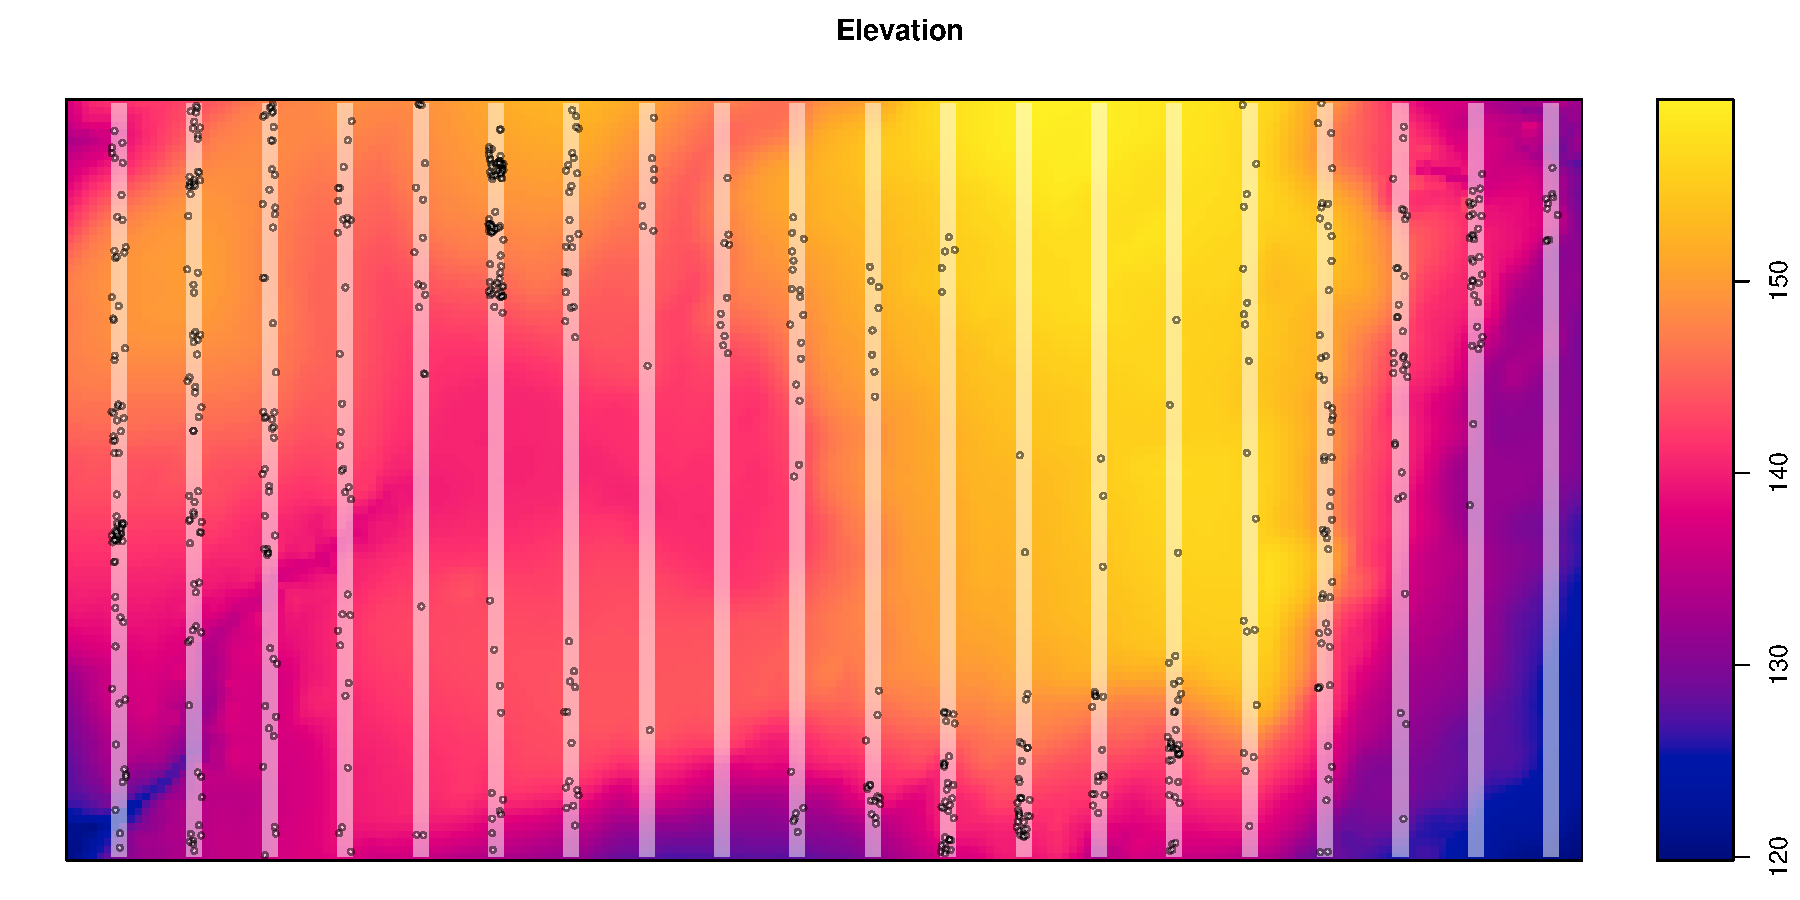
\includegraphics[width=0.9\textwidth]{figures/bei-effort_elev.pdf}}

\subfloat[Magnitude of the elevation gradient, with observed region and events
overlaid.]
{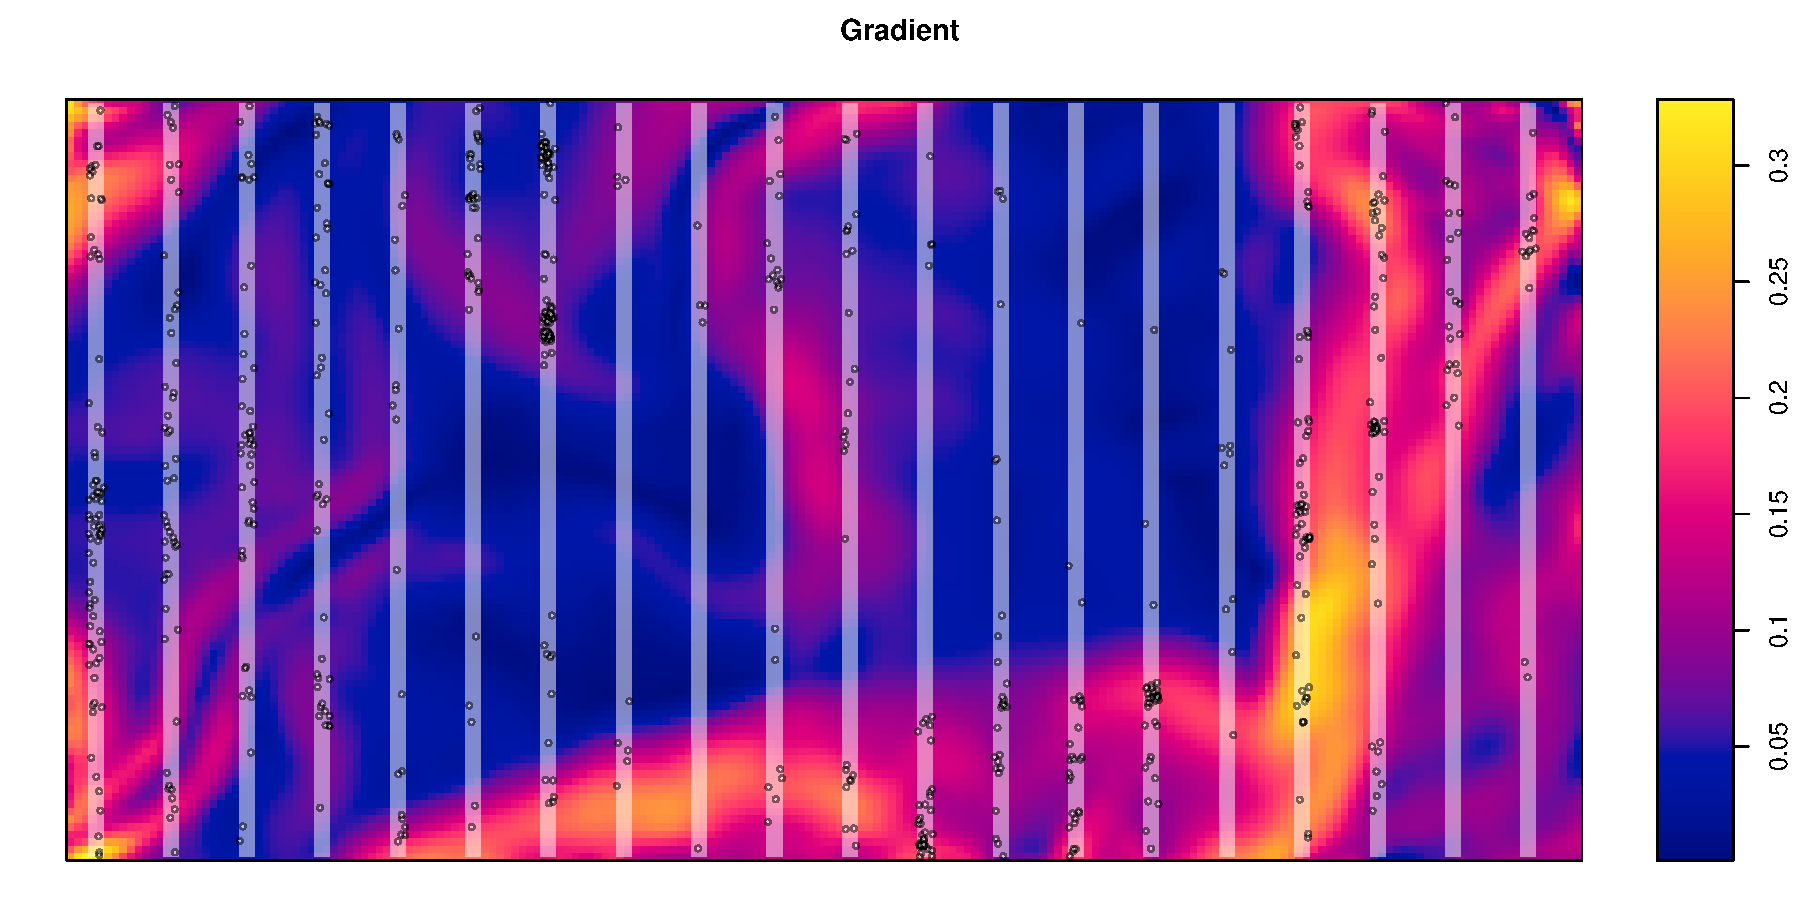
\includegraphics[width=0.9\textwidth]{figures/bei-effort_grad.pdf}}

\caption{Plots of the event and covariate data.}
\label{effort}
\end{figure}


\subsubsection{Fitting in R-INLA}

The procedure for fitting the LGCP model to variable sampling effort data is
the same as for fully-observed data except that the weight vector
\(\boldsymbol{\alpha}\) is different. Our code is available in the
supplementary materials.

The mesh~(Figure~\ref{effortmesh}) is the same as used with the fully-observed
point pattern, with \(m = 2145\) nodes. We interpolated the covariates
at the nodes and had \texttt{INLA} can initialize the covariance structure as
before. The pseudodata vector changes dimension, becoming
\begin{displaymath}
\mathbf{y} = (0, \dots, 0, 1, \dots, 1)'
\end{displaymath}
with 2145 zeros corresponding to the mesh nodes and 710 ones for the observed
events.

The computation of the weight vector is more involved. The notation is again
\begin{displaymath}
\boldsymbol{\alpha} = (\alpha_{1}, \dots, \alpha_{2145}, 0, \dots, 0)',
\end{displaymath}
now with 710 zeros representing the observed events. The alphas equal the
observed area represented by each node. We used tools from \texttt{spatstat}
to calculate these areas. First, we created an \texttt{owin} object defining
the observed region along the transects. Then, we created a list of
\texttt{owin} objects with each representing one triangle of the mesh. Next,
we intersected the observed region with each triangle to partition the observed
region into many small shards, each contained within a single
triangle~(Figure~\ref{effortpartition}). Then we calculated the area of each
shard. These areas are each associated with a triangle, but the need to be
allocated to the nodes at the vertices of the triangle. To do this, we found
the centroid of each shard and allocated the area proportional to the
barycentric coordinates of the centroid. This way, the area of each shard is
distributed to the three nodes which define the triangle, and the closest node
gets the most weight while the farthest node get the least weight. Finally,
the alpha value for each node is computed by summing the weights contributed
by each shard to that node.

{\it Is there a better (or more formal) term than ``shard''? It has an
intuitive meaning to me, but it feels weird to create nonstandard terminology
for use in exactly one paragraph. ---Kenny}

Finally, the pseudodata, covariates, and an index are combined into a data
list and the \texttt{inla()} function is called to fit the model.

\begin{figure}[h]
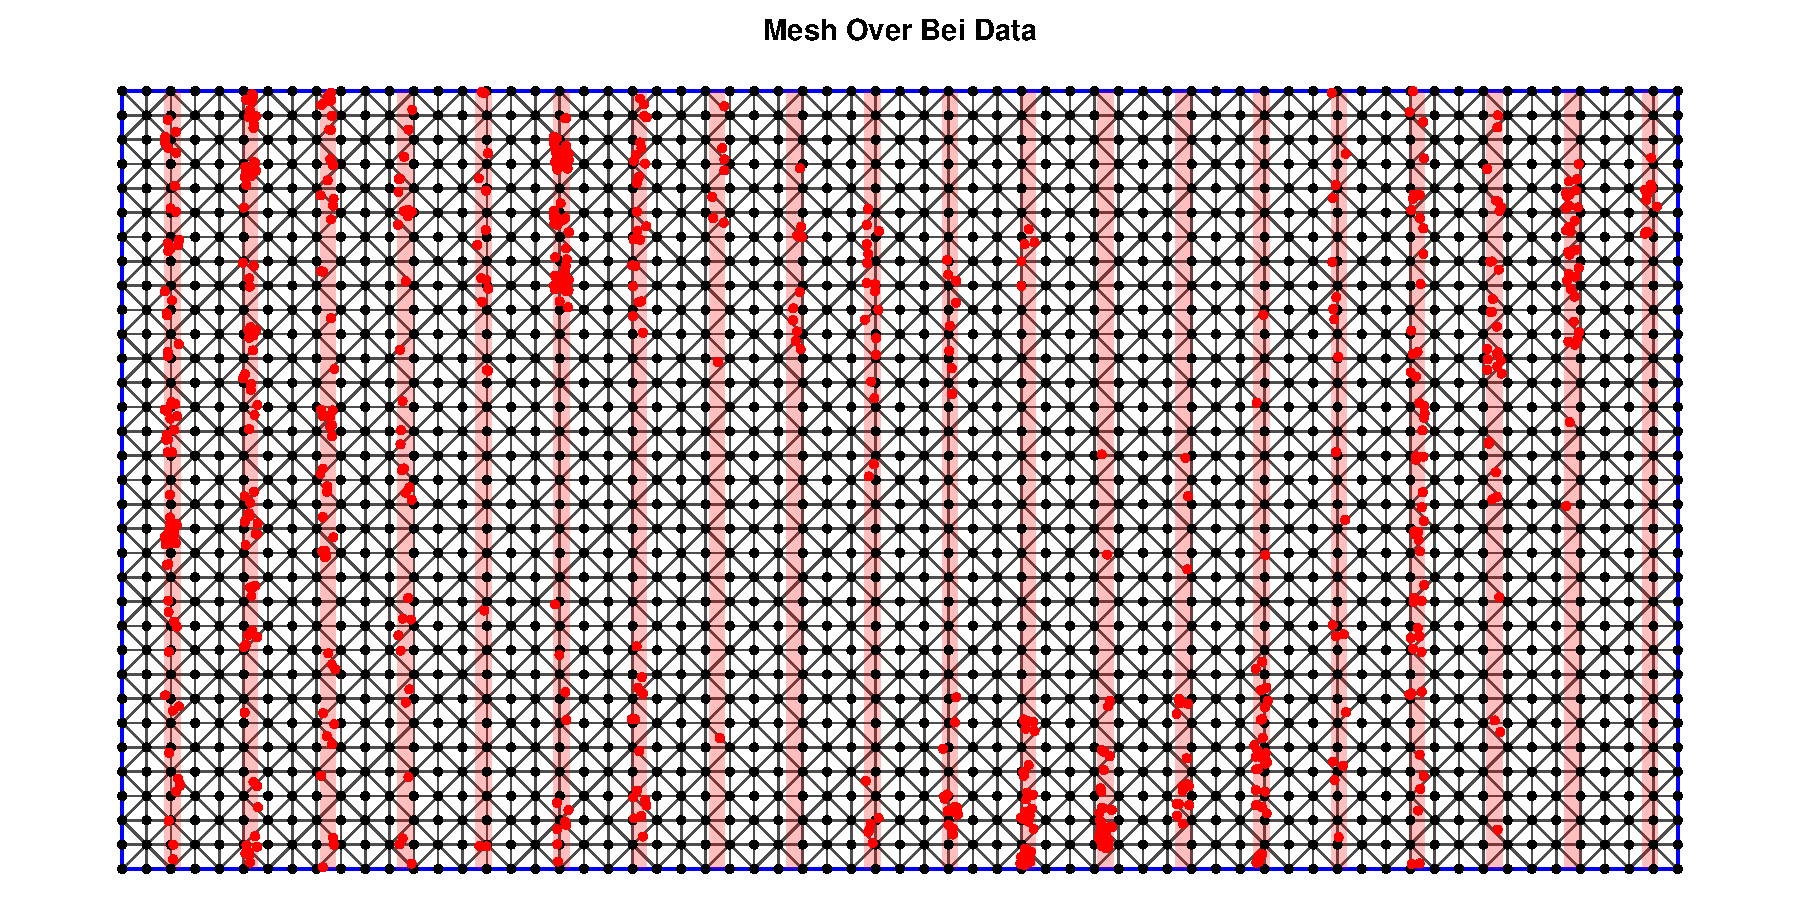
\includegraphics[width=\textwidth]{figures/bei-effort_mesh.pdf}
\caption{Triangular mesh with observed region and events overlaid.}
\label{effortmesh}
\end{figure}

\begin{figure}[h]
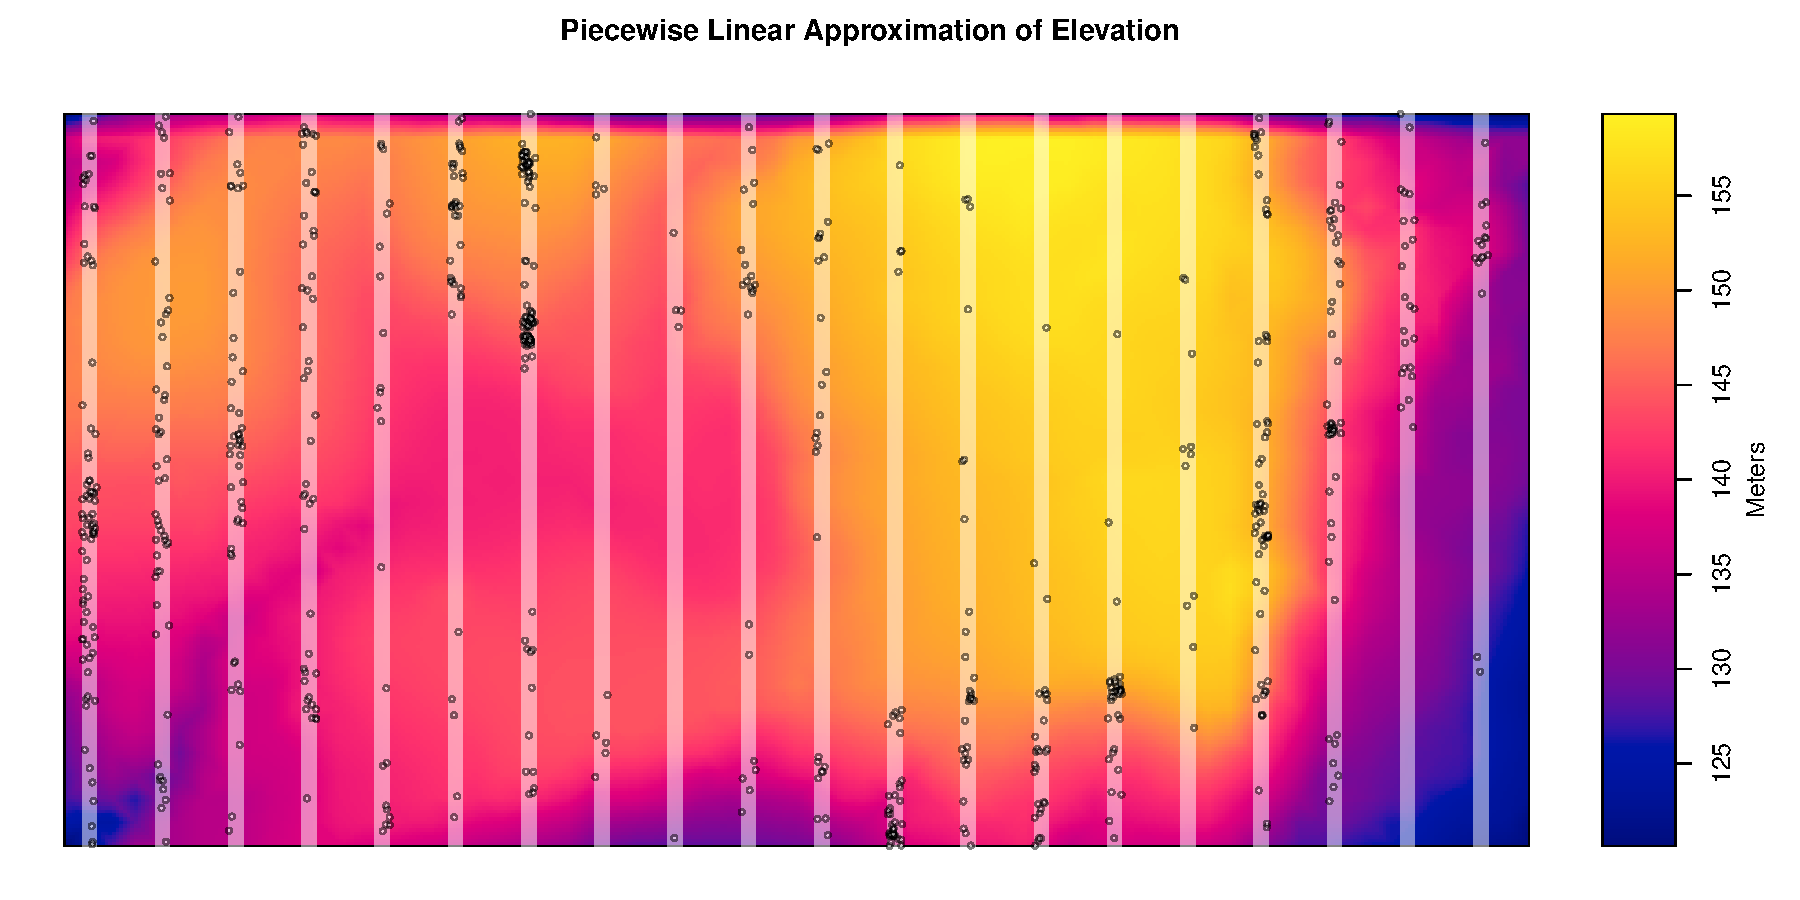
\includegraphics[width=\textwidth]{figures/bei-effort_elev_mesh.pdf}
\caption{Piecewise linear approximation of the elevation surface.}
\label{effortelevmesh}
\end{figure}

\begin{figure}[h]
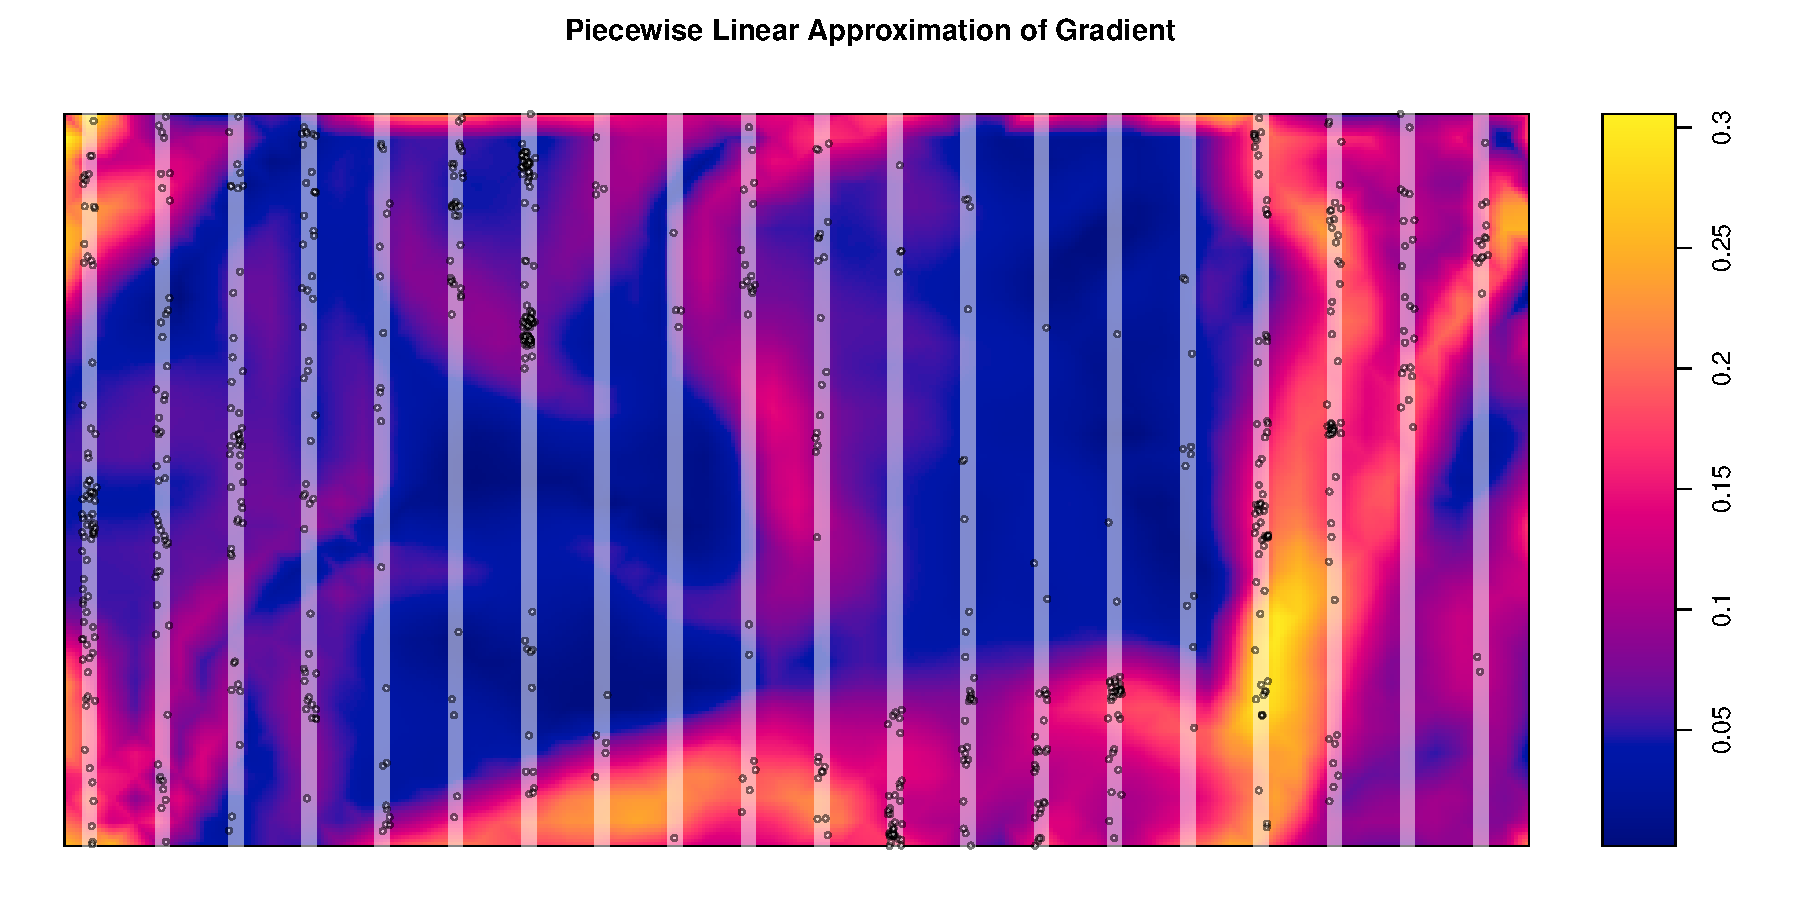
\includegraphics[width=\textwidth]{figures/bei-effort_grad_mesh.pdf}
\caption{Piecewise linear approximation of the gradient surface.}
\label{effortgradmesh}
\end{figure}

\begin{figure}[h]
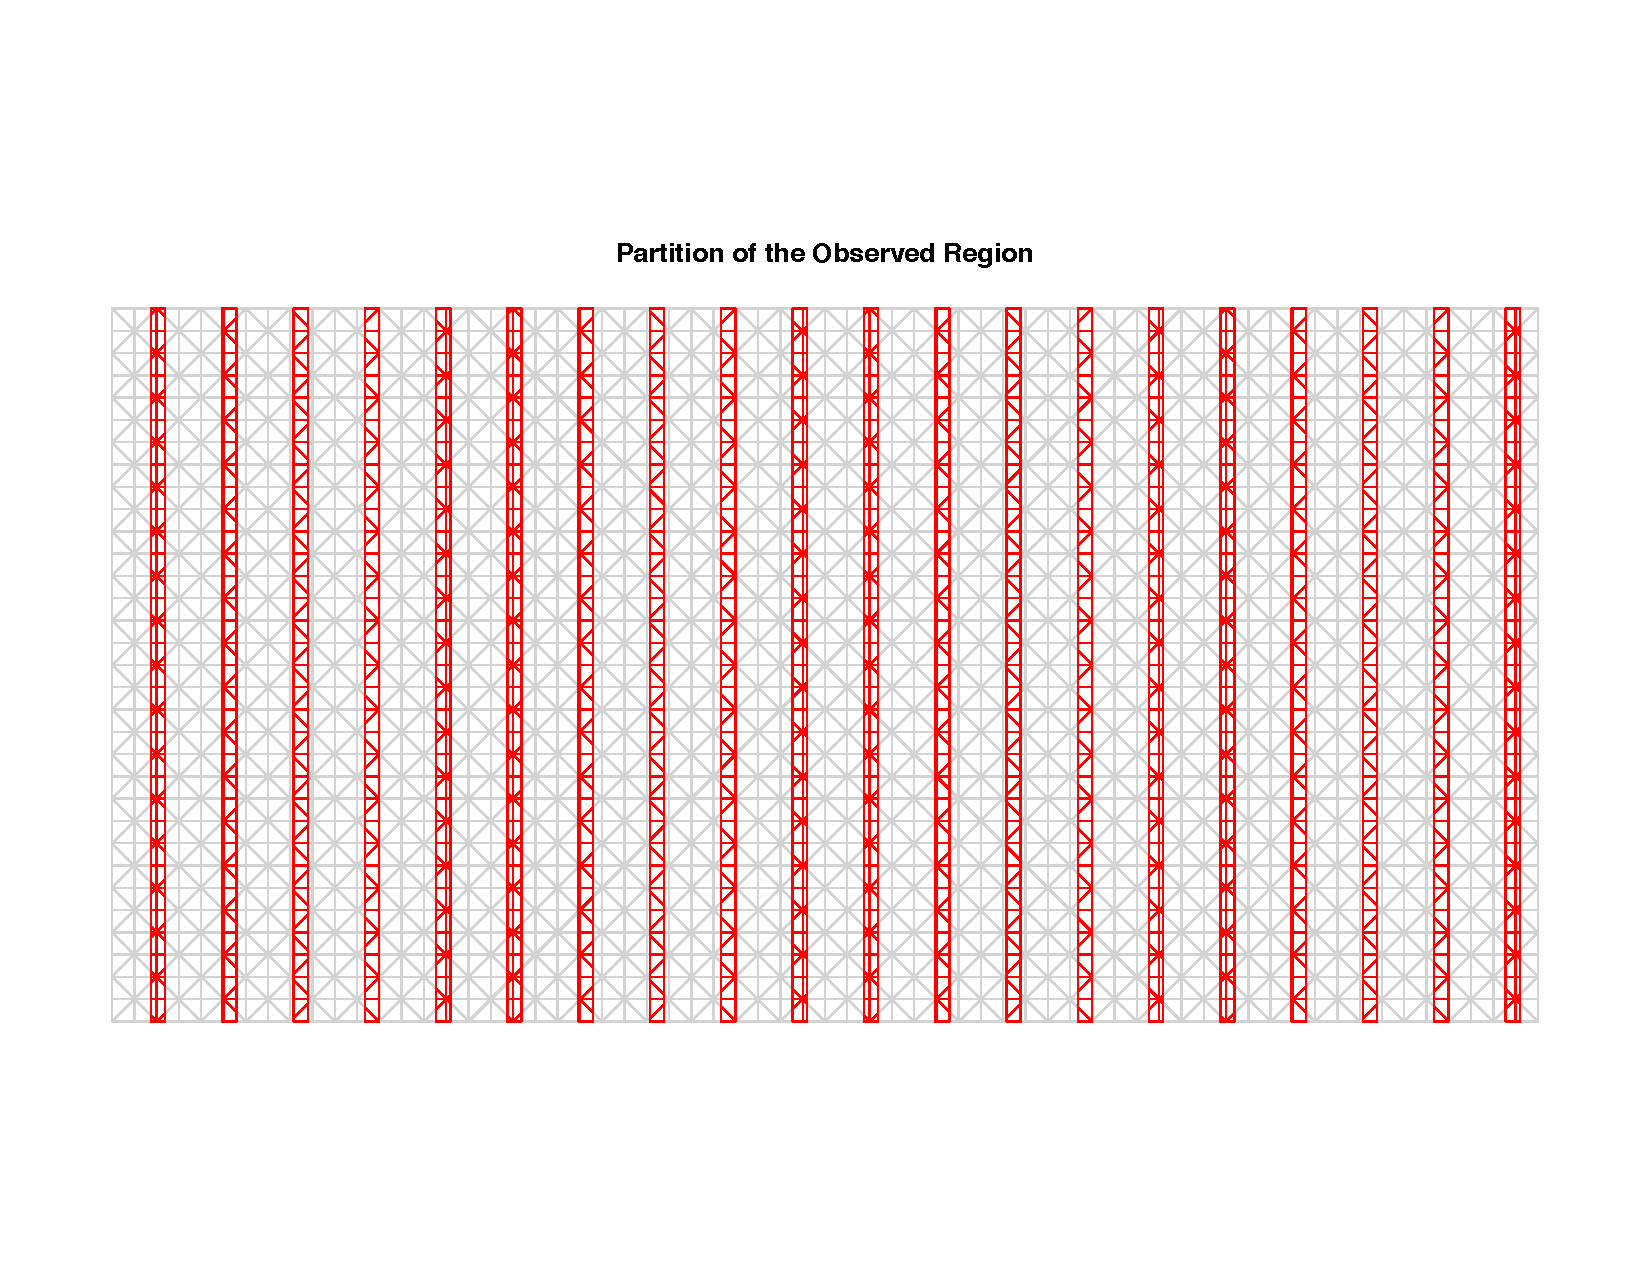
\includegraphics[width=\textwidth]{figures/bei-effort_partition.pdf}
\caption{Partition of the observed region created by intersection with each
mesh triangle.}
\label{effortpartition}
\end{figure}

\subsubsection{Results}

Posterior means and central 95\% posterior intervals:
\(\beta_{0}\): \(-12.7\), \((-18.7, -7.07)\);
\(\beta_{1}\): \(0.0445\), \((0.00676, 0.0839)\);
\(\beta_{2}\): \(6.19\), \((3.21, 9.19)\);
\(\sigma\): \(1.29\), \((0.967, 1.76)\);
Range: \(237\), \((162, 352)\)

{\it decide which of figures \ref{effortbetas}, \ref{effortmean},
\ref{effortsd}, \ref{effortintensity} are needed, then combine into a single
multi-panel figure.}

The posterior mean of the fixed effect component of the linear predictor,
again appears very as an average of the elevation and gradient
surfaces~(Figure~\ref{effortbetas}), very similar to the previous figure. As
before, there is some additional spatial structure described by the
GP~(Figure~\ref{effortmean}). However, the predicted GP surface is smoother
compared to the model fit to the fully data.
{\it (compare posterior dists of covariance params)}

\begin{figure}[h]
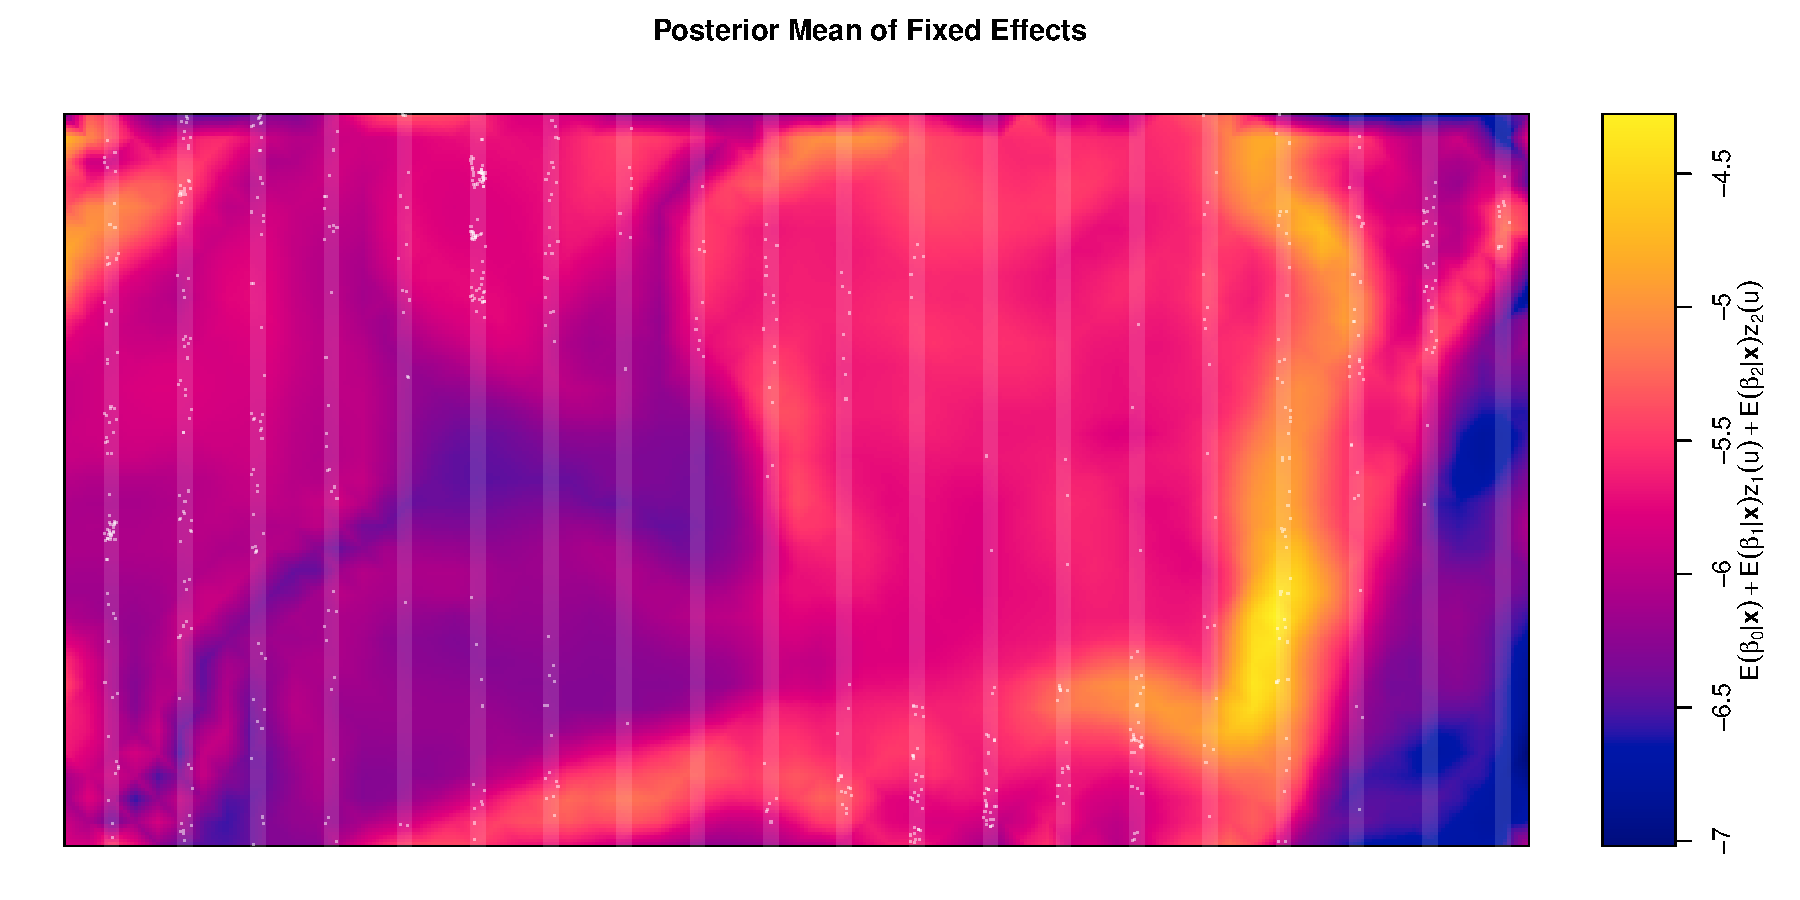
\includegraphics[width=\textwidth]{figures/bei-effort_betas.pdf}
\caption{Posterior mean surface for the fixed effects.}
\label{effortbetas}
\end{figure}

\begin{figure}[h]
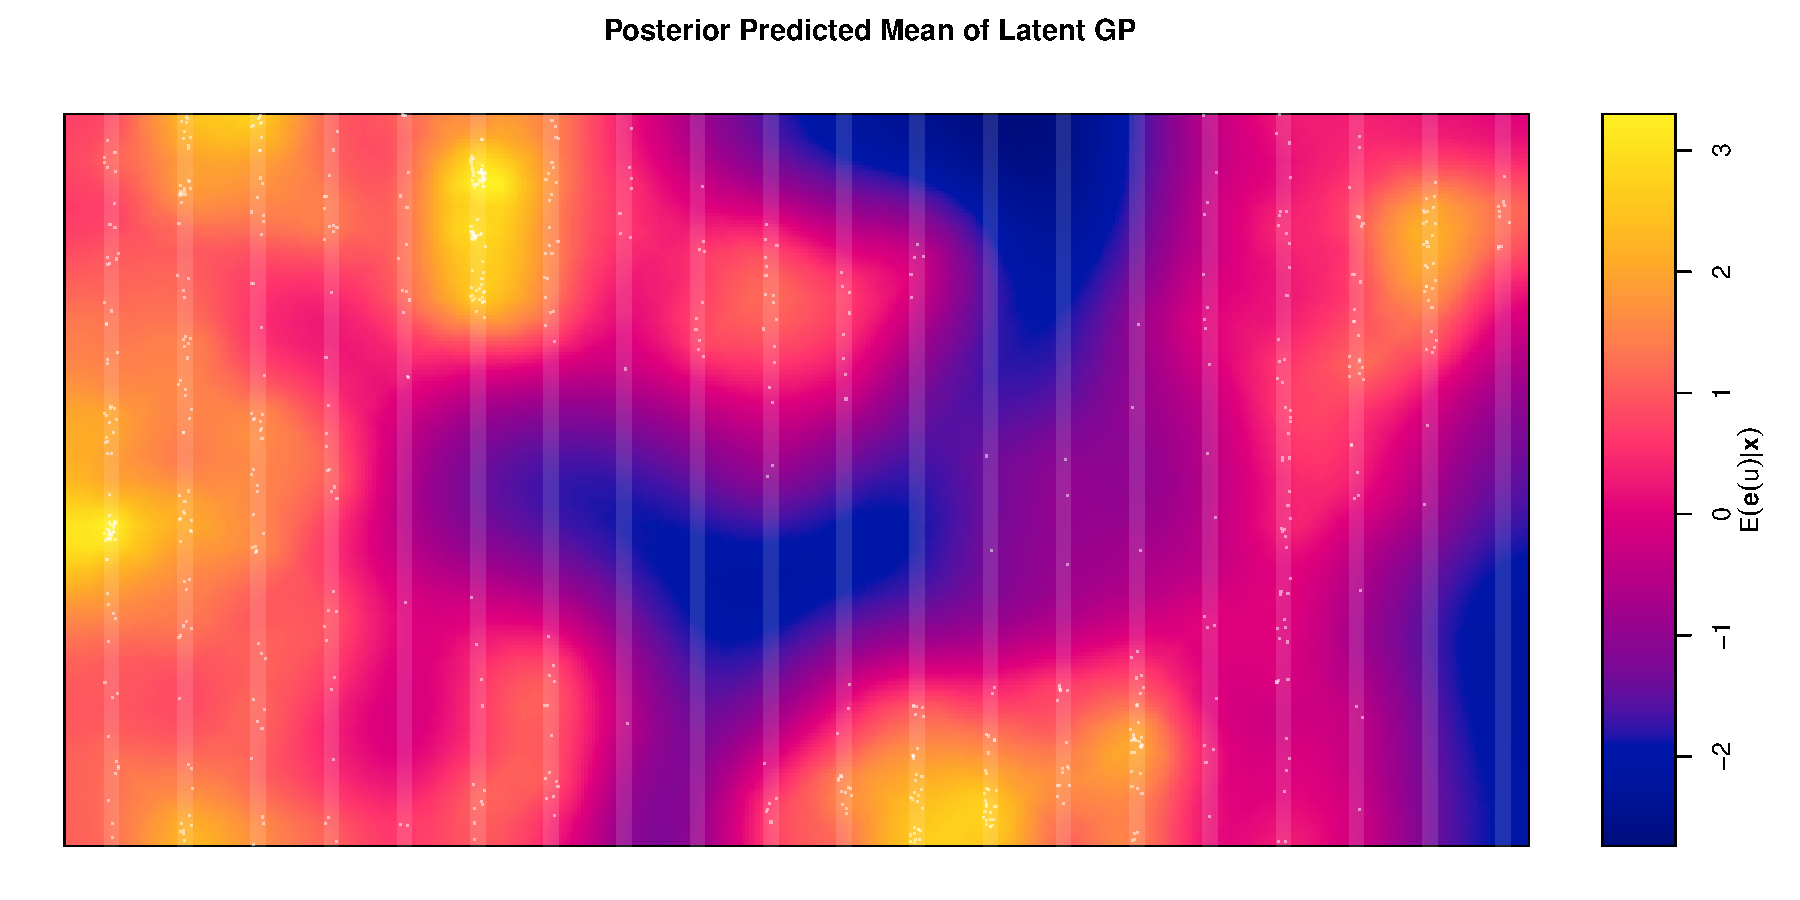
\includegraphics[width=\textwidth]{figures/bei-effort_mean.pdf}
\caption{Posterior mean of prediction surface.}
\label{effortmean}
\end{figure}

\begin{figure}[h]
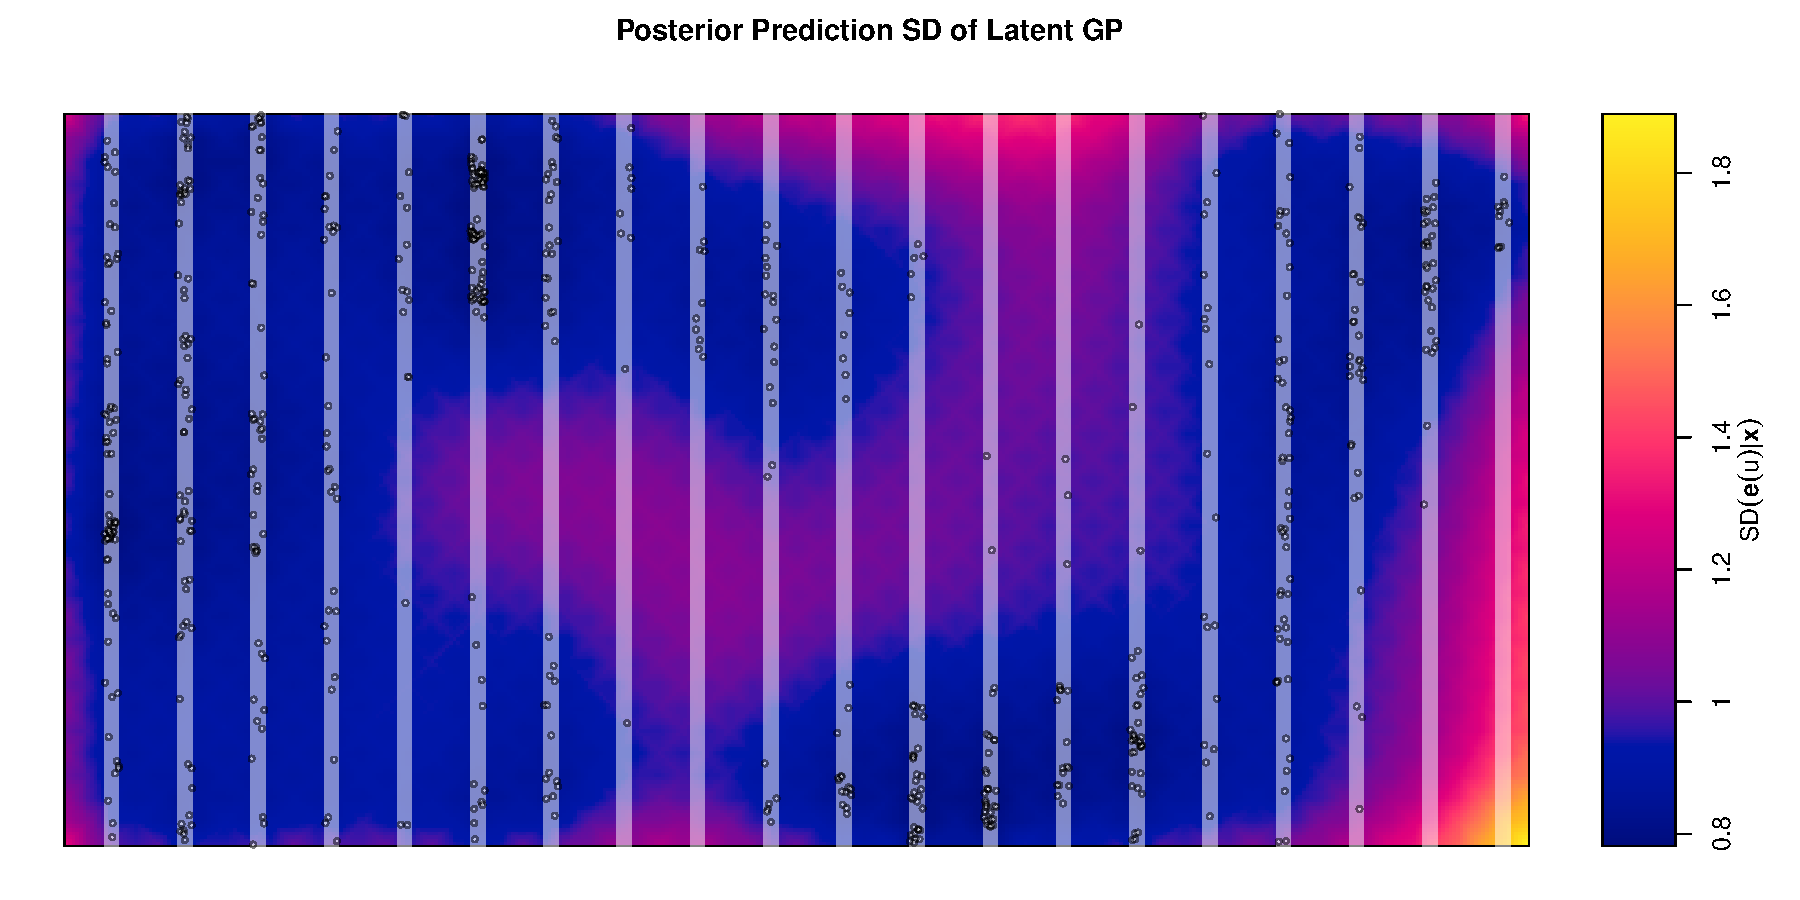
\includegraphics[width=\textwidth]{figures/bei-effort_sd.pdf}
\caption{Pointwise posterior standard deviation of predictions.}
\label{effortsd}
\end{figure}

\begin{figure}[h]
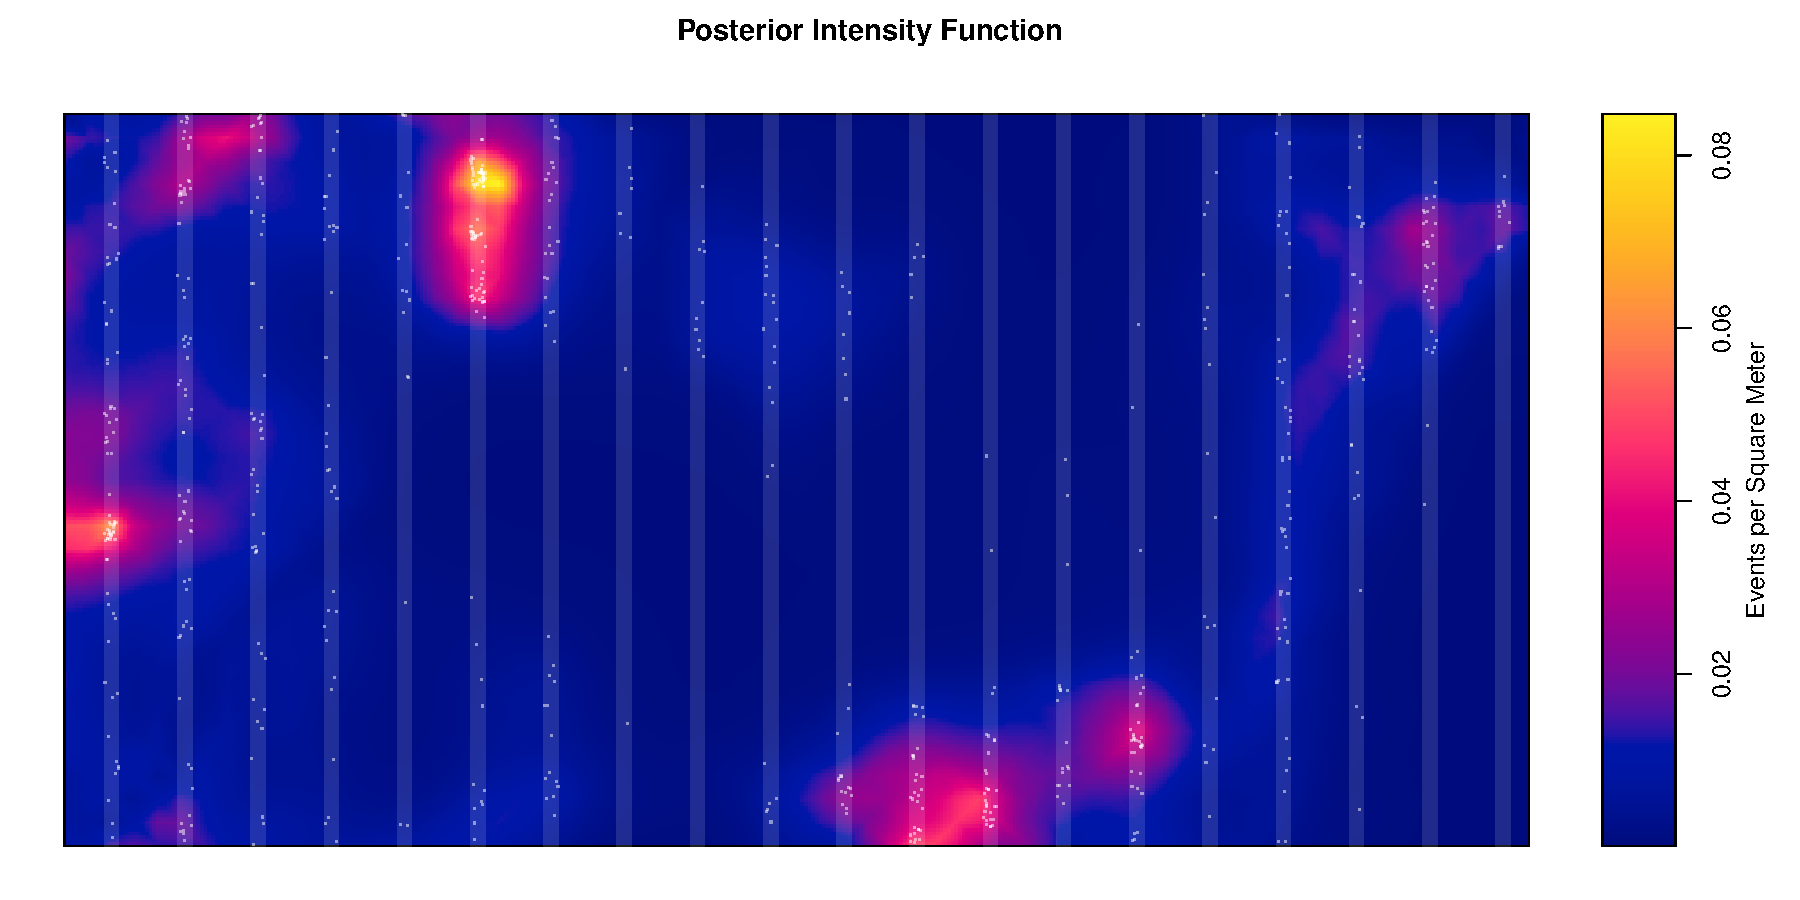
\includegraphics[width=\textwidth]{figures/bei-effort_intensity.pdf}
\caption{Posterior intensity surface in events per square meter, calculated
using the piecewise linear approximate covariate surfaces and the posterior
means of the intercept, coefficients, and GP.}
\label{effortintensity}
\end{figure}


\subsubsection{Model Checking}

\begin{figure}[h]
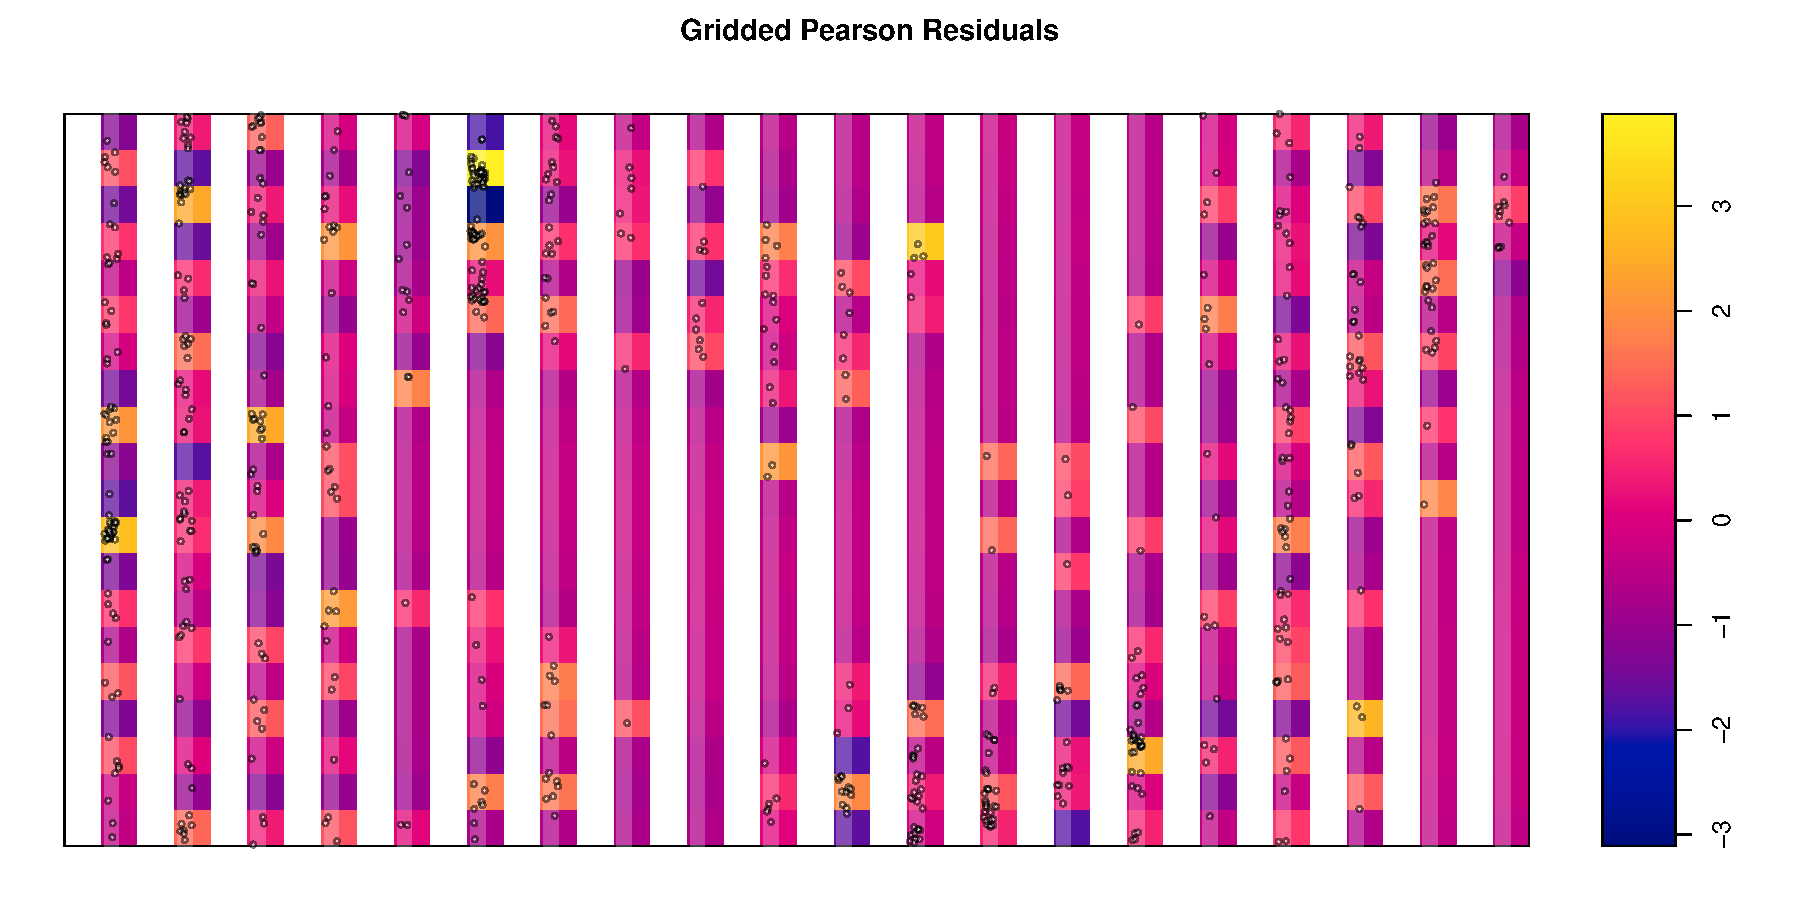
\includegraphics[width=\textwidth]{figures/bei-effort_residuals.pdf}
\caption{Pearson residuals calculated on a grid.}
\label{effortresiduals}
\end{figure}

Pearson residuals~(Figure~\ref{effortresiduals}): undefined where grid cells
have 0 observed area (because 0 events expected), where defined the residuals
appear similar to those from the model fit to the full data, small magnitude
in the observed region with no events and low posterior intensity, more large
positive residuals than large-magnitude negative residuals, random with no
obvious spatial patterns


\section{Conclusion and Discussion}
\label{conclusion}
%  {\bf Conclusion and Discussion:} In this conclusion and discussion section, provide conclusions of your review and provide anticipated future direction(s) in this area.

not really possible to get a posterior distribution of the intensity function
because it is a nonlinear transformation of several parameters and we do not
have their joint posterior

the mesh used for \texttt{bei} for is finer than needed to describe the
GP --- think about coarsening and refining based on the detail needed to
represent the covariates (is there literature on this?)

comment on similarities in posterior between model fit to full data and model
fit to sampled data

need further work on model checking when prediction is desired over a different
region than observed

shows that mapping based on Bayesian LGCP models is now practical with
useful accuracy in short amount of time


%\section*{Acknowledgement(s)}

%An unnumbered section, e.g.\ \verb"\section*{Acknowledgements}", may be used for thanks, etc.\ if required and included \emph{in the non-anonymous version} before any Notes or References.

%\section*{Disclosure statement}

%An unnumbered section, e.g.\ \verb"\section*{Disclosure statement}", may be used to declare any potential conflict of interest and included \emph{in the non-anonymous version} before any Notes or References, after any Acknowledgements and before any Funding information.

%\section*{Funding}

%An unnumbered section, e.g.\ \verb"\section*{Funding}", may be used for grant details, etc.\ if required and included \emph{in the non-anonymous version} before any Notes or References.

%\section*{Notes on contributor(s)}

%An unnumbered section, e.g.\ \verb"\section*{Notes on contributors}", may be included \emph{in the non-anonymous version} if required. A photograph may be added if requested.

%\section*{Nomenclature/Notation}

%An unnumbered section, e.g.\ \verb"\section*{Nomenclature}" (or \verb"\section*{Notation}"), may be included if required, before any Notes or References.

%\section*{Notes}

%An unnumbered `Notes' section may be included before the References (if using the \verb"endnotes" package, use the command \verb"\theendnotes" where the notes are to appear, instead of creating a \verb"\section*").

\bibliographystyle{tfs}
\bibliography{jas-inla-review}

\end{document}
